\chapter{Kinematics of the Charmless Three-Body Decay \texorpdfstring{\decay{\Lb}{\Lz\Kp\Km}}{Λb → ΛKK}}
The charmless three-body decay \decay{\Lb}{\Lz\Kp\Km} appears as a peaking background in $m(\Dz\Lz)$ if not sufficiently suppressed.
In Sec.~\ref{sec:bkgs_charmless} we establish such a suppression and benefit from some particular kinematic features we want to discuss in this chapter.
First, we discuss the distribution of the reflected mass $m(\Lz\Km\pip)$ in Sec.~\ref{sec:apdx_charmlessrefl_mass} and introduce some notation.
We then study the momentum distribution of the \Lz baryon in Sec.~\ref{sec:apdx_charmlessrel_Lzp} which leveraged the strong separation power of the \Lz classifier.

\section{Mass Distributions}
\label{sec:apdx_charmlessrefl_mass}
For describing the relativistic kinematic of three-body decays $\decay{M}{1\,2\,3}$ one often uses combined squared masses of two daughters, \eg{}, $m_{12}^2$.
Following the notation of the \gls{pdg}, these squared masses are given by the four momenta $p_i$ of the daughters
\begin{equation*}
    m^2_{ij} := \left( p_i + p_j \right)^2 \,, \\
\end{equation*}
and obey useful relations, such as
\begin{equation}
    \label{eq:apdx_charmelssrefl_mijsum}
    m_{12}^2 + m_{23}^2 + m_{13}^2 = M^2 + m_1^2 + m_2^2 + m_3^2 \,,
\end{equation}
where $M$ ($m_i$) refers to the mass of the decaying mother (daughter $i$).
Eq.~\eqref{eq:apdx_charmelssrefl_mijsum} can be rewritten
\begin{equation*}
    m_{12}^2 = M^2 + m_3^2 - 2ME_3 \,,
\end{equation*}
where $E_3$ is the energy of particle 3 in the rest frame (CMS) of $M$ and thus allows the determination of the kinematic boundaries of $m_{ij}^2$, \eg{},
\begin{align*}
    \operatorname{max} m_{23}^2 &= \left( E_2^* + E_3^* \right)^2 - \left( \sqrt{ \left( E_2^* \right)^2 - m_2^2} - \sqrt{ \left( E_3^* \right)^2 - m_3^2} \right)^2 \,, \\
    \operatorname{min} m_{23}^2 &= \left( E_2^* + E_3^* \right)^2 - \left( \sqrt{ \left( E_2^* \right)^2 - m_2^2} + \sqrt{ \left( E_3^* \right)^2 - m_3^2} \right)^2 \,,
\end{align*}
where
\begin{align*}
    E_2^* &= \frac{m_{12}^2 - m_1^2 + m_2^2}{2 m_{12}} \quad \text{and} \\
    E_3^* &= \frac{M^2 - m_{12}^2 - m_3^2}{2 m_{12}}
\end{align*}
are the energies of particle~2 and 3 in the rest frame of $m_{12}$.

In the context of, the present analysis the three-body decay \decay{\Lb}{\Lz\Km\Kp} appears as a (non-resonant) \gls{reflection} in the $m(\Dz\Lz)$ distribution.
More generally, a \gls{reflection} occurs if w.l.o.g.\ particle 3 with genuine mass $m_3$ is reconstructed using the spurious mass hypothesis $m_x$.
If so, the reconstructed invariant mass of the mother in the CMS $\tilde{M}_\text{cms}$ is given by
\begin{multline*}
    \tilde M_\text{cms} = \sqrt{m_1^2 + \vec{p}_1^{\,2}} + \sqrt{m_2^2 + \vec{p}_2^{\,2}} + \sqrt{m_x^2 + \vec{p}_3^{\,2}} \\
    = \frac{M^2 + m_1^2 - m_{23}^2}{2M} + \frac{M^2 + m_2^2 - m_{13}^2}{2M} + \sqrt{ \left( \frac{M^2 + m_3^2 - m_{12}^2}{2M} \right)^2 - m_3^2 + m_x^2}
%    = \frac{M^2 - m_3^2 + m_{12}^2}{2M} + \sqrt{ \left( \frac{M^2 + m_3^2 - m_{12}^2}{2M} \right)^2 - m_3^2 + m_x^2}
\end{multline*}
and thus
\begin{equation}
    \label{eq:apdx_charmlessrefl_Mcms}
    \tilde M_\text{cms} \left(m_{12}^2 | m_x \right) = \frac{M^2 - m_3^2 + m_{12}^2}{2M} + \sqrt{ \left( \frac{M^2 + m_3^2 - m_{12}^2}{2M} \right)^2 - m_3^2 + m_x^2} \,.
\end{equation}
We note two things:
First, only if $m_x = m_3$ then $\tilde M_\text{cms} = M$ for any frame of reference.
Otherwise, Eq.~\eqref{eq:apdx_charmlessrefl_Mcms} only holds in the CMS of $M$.
Secondly, if the invariant mass is determined in the laboratory system whilst already assuming the spurious mass hypothesis, then the energy and thus the boost of the respective particle is also wrong.
In this case, this will result in a smearing due to the inaccurate boosting of $\tilde{M}_\text{cms}$, degrading Eq.~\eqref{eq:apdx_charmlessrefl_Mcms} to an approximation rather than an exact solution.

In Fig.~\ref{fig:apdx_charmlessrefl_dalitz} we show the Dalitz plot~\cite{dalitz1,dalitz2} of $m^2_{23} = m^2_{\kaon\kaon}$ and $m^2_{12} = m^2_{\Lz\Km}$, as well as the correlation of $m^2_{12}$ with the reflected mass $m(\Lz\Km\pip)$ together with the approximate solution Eq.~\eqref{eq:apdx_charmlessrefl_Mcms}.
\begin{figure}[htbp]
    \centering
    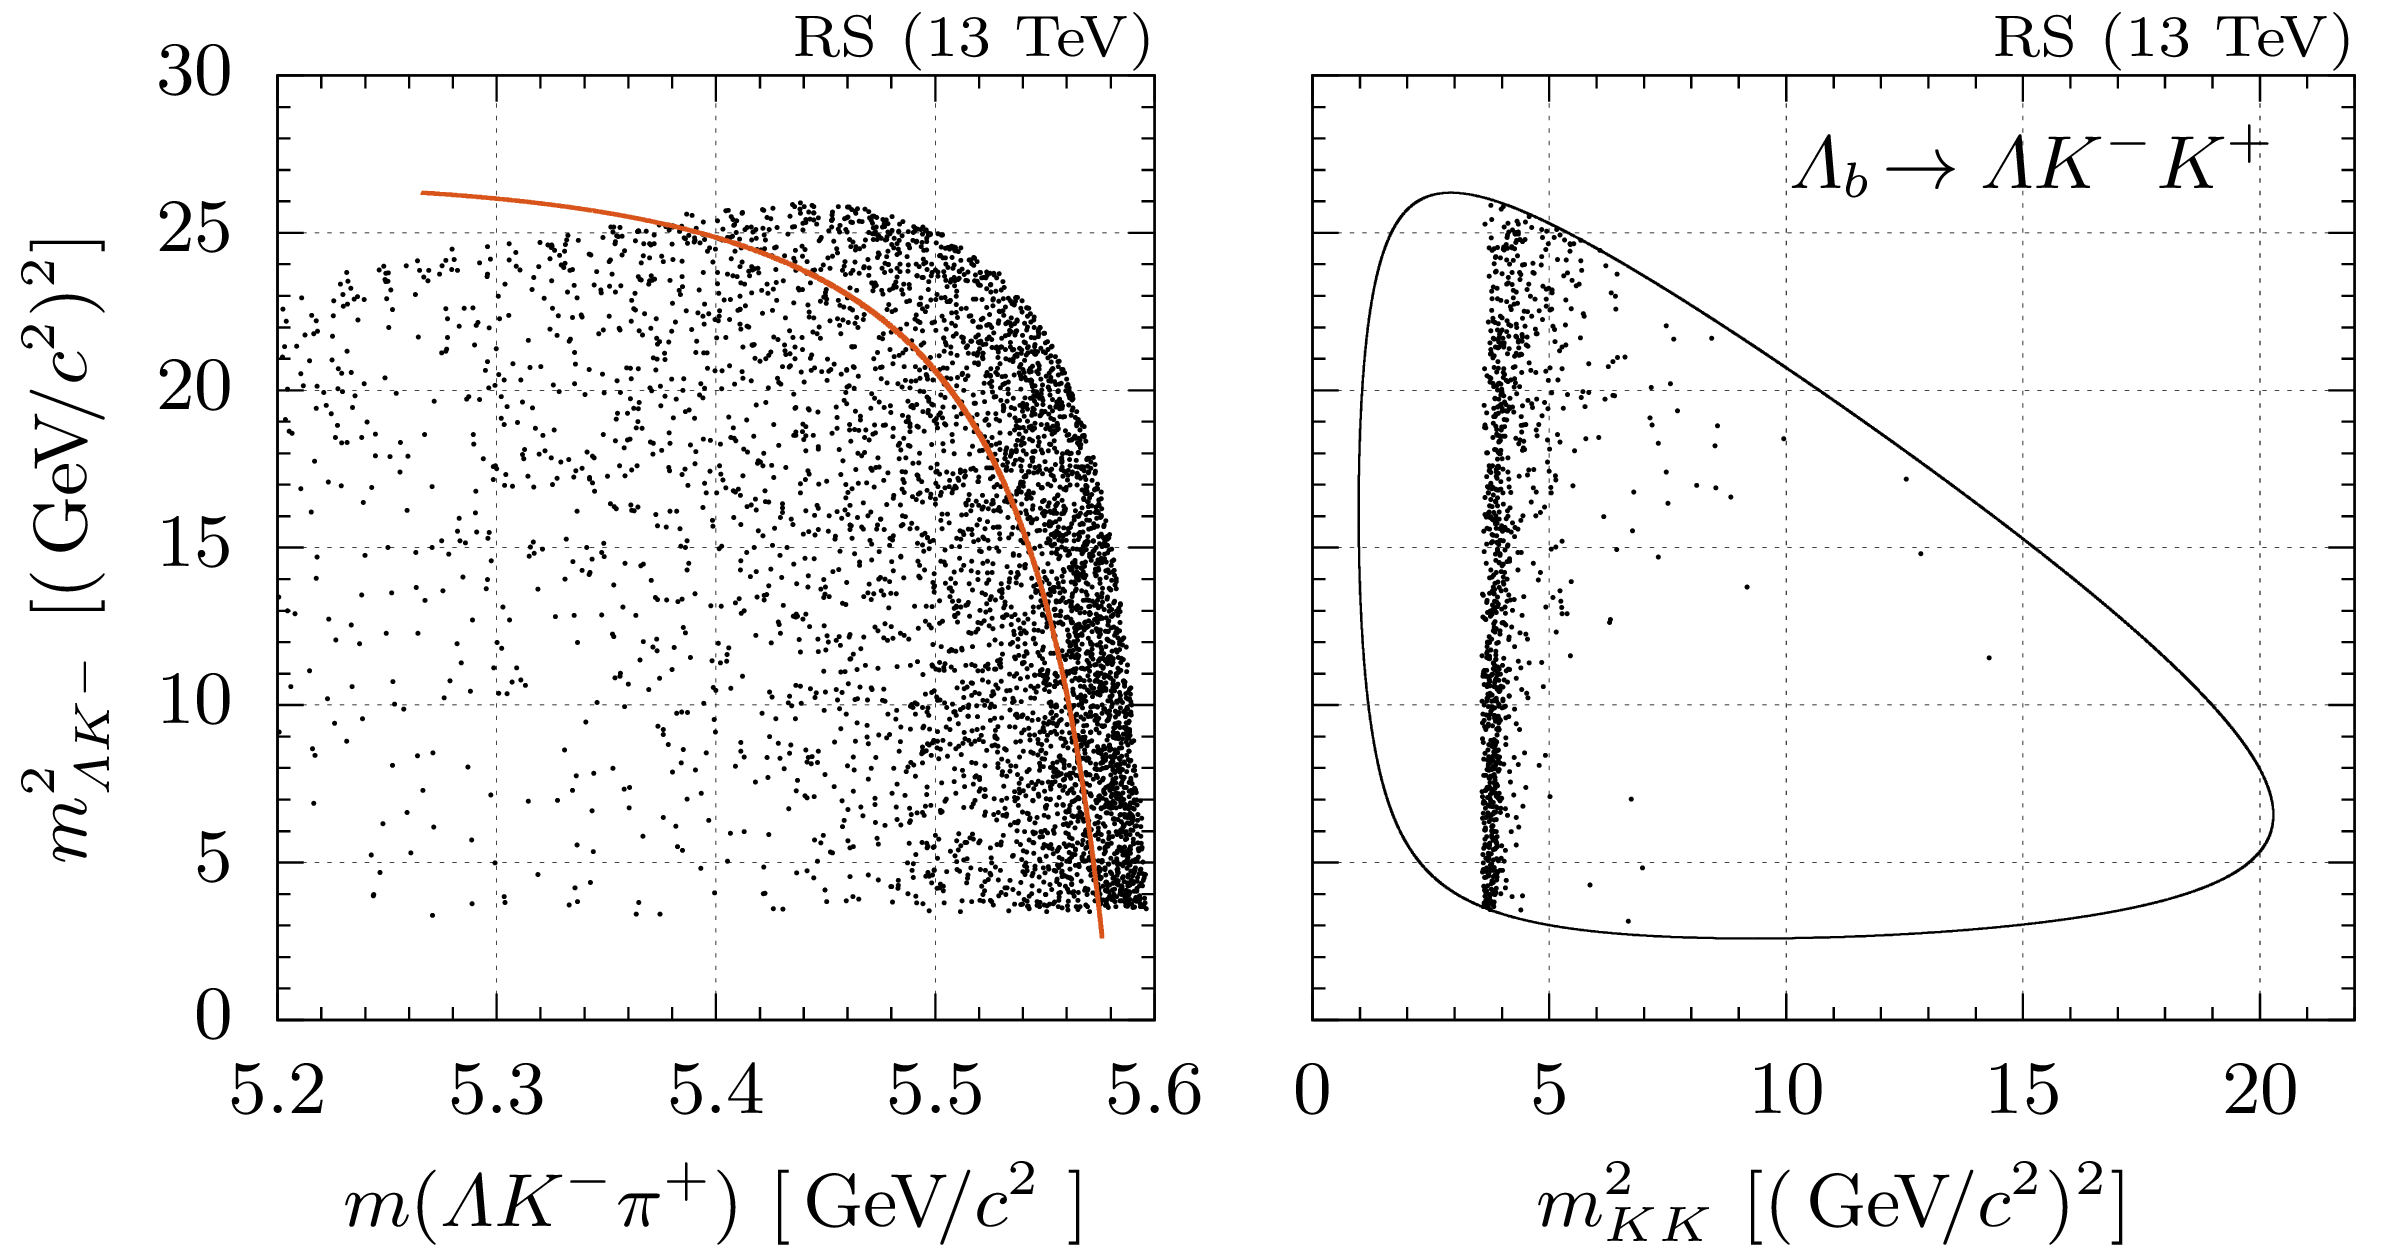
\includegraphics[scale=1.]{Lb2LzKK_bkg/dalitz.png}
    \caption{Dalitz plot (right) of $m^2_{23} = m^2_{\kaon\kaon}$ and $m^2_{12} = m^2_{\Lz\Km}$, as well as the correlation of $m^2_{12}$ with the reflected mass $m(\Lz\Km\pip)$ using simulated data (left). The solid, orange line on the left indicates the reflected invariant $\tilde M_\text{cms}$ in the CMS of $M$, according to Eq.~\eqref{eq:apdx_charmlessrefl_Mcms}. The data are filtered w.r.t.\ the (smeared) vicinity of $m_{2x}^2=m^2_{\Km\pip}$ to the \Dz mass.}
    \label{fig:apdx_charmlessrefl_dalitz}
\end{figure}
The data points are calculated from unsmeared values taken from simulations with the framework \texttt{RapidSim}~\cite{rapidsim} and filtered w.r.t.\ the (smeared) vicinity of $m_{2x}^2=m^2_{\Km\pip}$ to the \Dz mass.
(See Ref.~\cite{LbToLzhh} for Dalitz plots from recorded data. Given the limited data sample, resonance structures are not obvious to identify, however, known \Lb decays, such as \decay{\Lb}{\Lz\Pphi}~\cite{LbToLzphi}, are well separated in $m^2_{\kaon\kaon}$.)
The distribution of the invariant mass $m(\Lz\Km\pip)$ in the CMS is (approximately) proportional to the product of the inverted derivative of Eq.~\eqref{eq:apdx_charmlessrefl_Mcms} (solid line in the left part of Fig.~\ref{fig:apdx_charmlessrefl_dalitz}) and the density of $m^2_{12} \equiv m^2_{\Lz\Km}$, where the latter is flat for the central part of $m^2_{\Lz\Km}$, due to the narrow mass range centered around the $m(\Dz)$ mass.
At the sharp edges of the Dalitz distribution (\ie{}, the kinematic boundaries) $m^2_{\Lz\Km}$ gets sliced, resulting in a smearing of $m(\Lz\Km\pip)$.
The peak in the $m(\Lz\Km\pip)$ distribution (\cf{}~Fig.~\ref{fig:LbToLzKK_bkg_hLbM}), caused by the steepness of the inverted derivative of Eq.~\eqref{eq:apdx_charmlessrefl_Mcms}, is thus naturally smeared.
We note that this smearing is often exclusively and imprecisely attributed to \textit{resolution effects} of the apparatus but in fact is an admixture of the outlined natural smearing in the CMS, a broadening due to boosting and eventually due to the quoted resolution effects.

\section{Kinematics of the \texorpdfstring{\Lz}{Λ} Baryon in Two and Three-Body Decays}
\label{sec:apdx_charmlessrel_Lzp}
Na\"ively, one might not expect major deviations between the kinematics of the \Lz baryon in the \decay{\Lb}{\Dz\Lz} decay and its charmless counterpart.
However, we saw deviations in the respective \pt distributions in Sec.~\ref{sec:bkgs_charmless} and saw the \Lz classifier picking up this deviation to effectively separate between both decays.

In Fig.~\ref{fig:apdx_charmlessrefl_pLz} we show the three-momentum magnitudes of \Lz baryons in the \Lb rest frame.
For the two-body decays \decay{\Lb}{\Dz\Lz}, this value is a $\delta$-spike (dashed line in Fig.~\ref{fig:apdx_charmlessrefl_pLz}), sitting at 
\begin{equation*}
    p^* = \sqrt{ \frac{ \left[ m_{\Lb}^2 - (m_{\Dz} + m_{\Lz})^2 \right] \left[ m_{\Lb}^2 - (m_{\Dz} - m_{\Lz})^2 \right]}{4m_{\Lb}^2}} \,,
\end{equation*}
whereas in three-body decays the distribution is broad.
The maximal value in the latter case corresponds to the configuration where the \Lz goes back-to-back with the $\Ph\Ph'$ pair of the respective \decay{\Lb}{\Lz\Ph\Ph'} pair, allowing slightly larger values if $m_{\Ph} + m_{\Ph'} < m_{\Dz}$, but the majority of configurations results in values below $p^*$ as shown in Fig.~\ref{fig:apdx_charmlessrefl_pLz}.
\begin{figure}[htbp]
    \centering
    \begin{subfigure}{.49\textwidth}
        \centering
        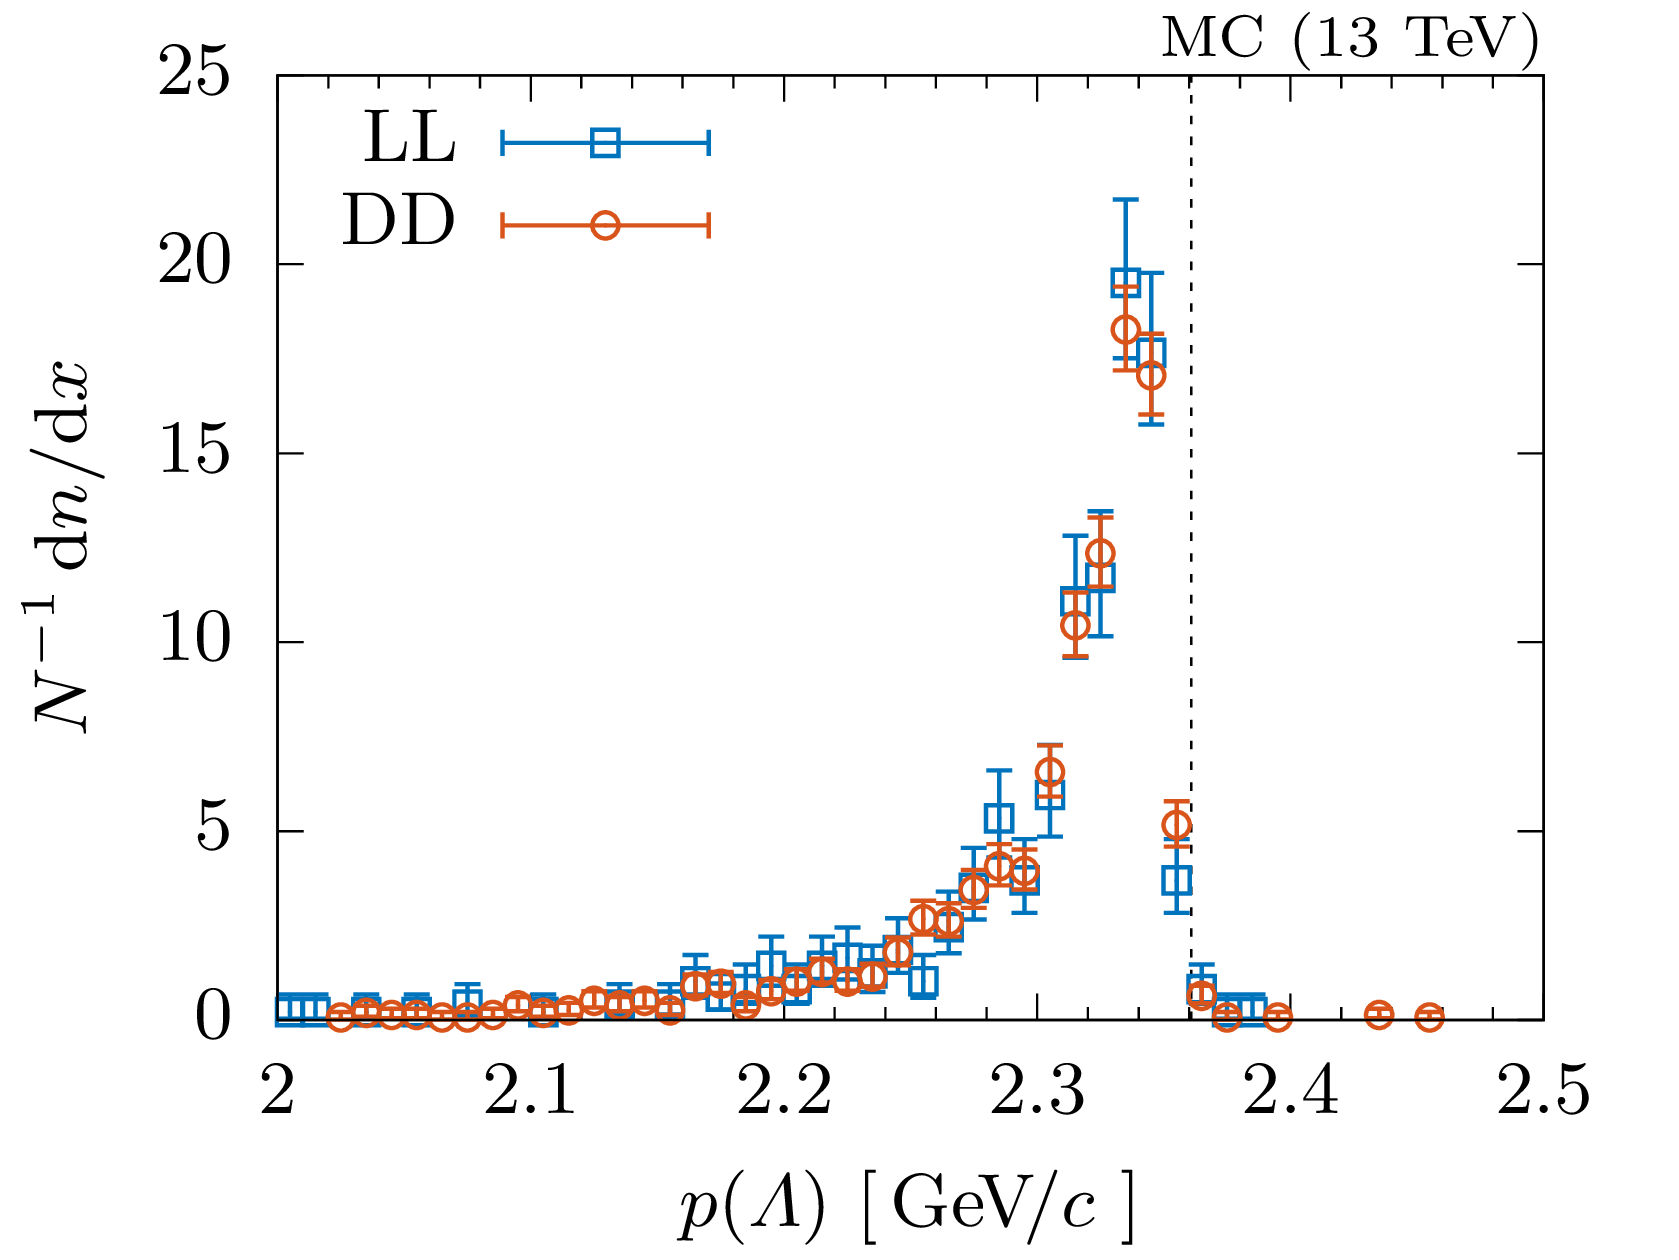
\includegraphics[scale=1.]{Lb2LzKK_bkg/hpLz_cms_Lb2LzKK_true.png}
    \end{subfigure}
    \begin{subfigure}{.49\textwidth}
        \centering
        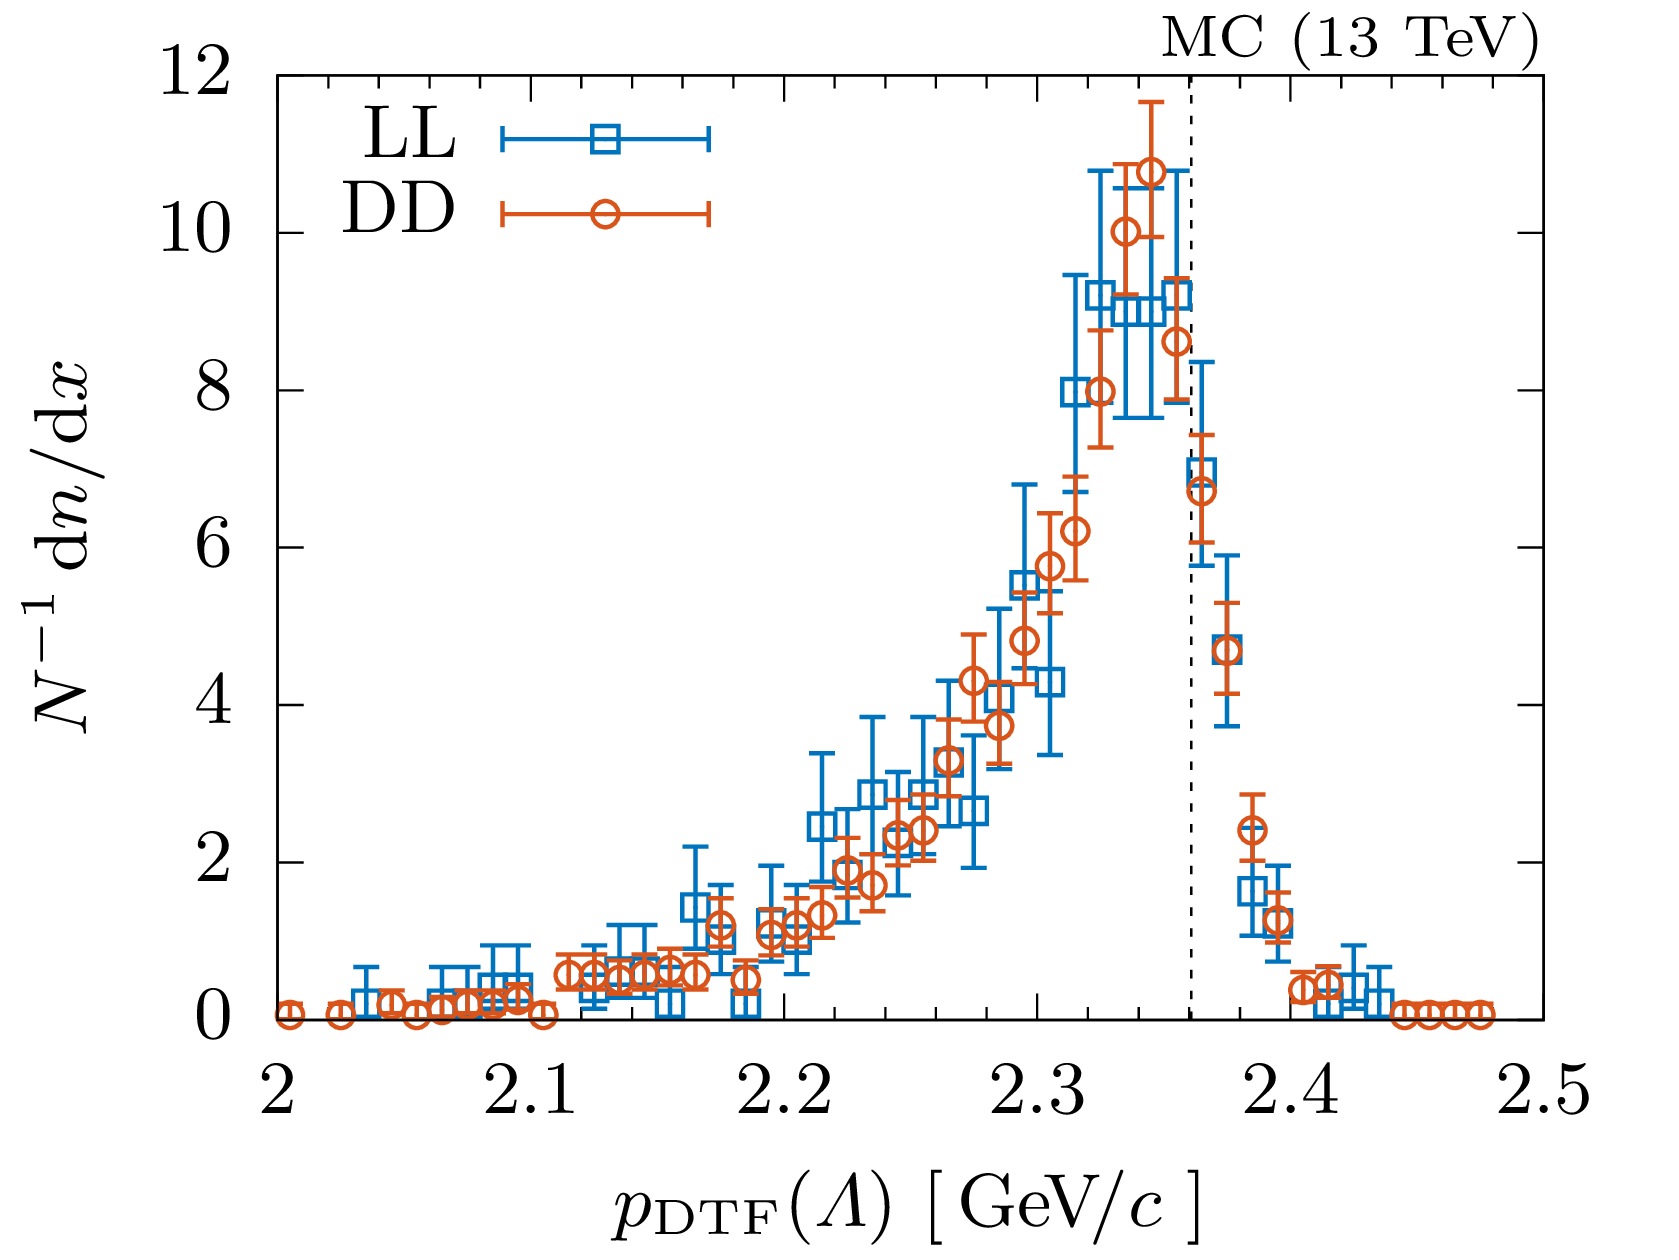
\includegraphics[scale=1.]{Lb2LzKK_bkg/hpLz_cms_Lb2LzKK_dtf.png}
    \end{subfigure}
    \caption{Distribution of three-momentum magnitudes of \Lz baryons in the \Lb rest frame for \gls{LL} and \gls{DD} tracks for \gls{mc} simulated \decay{\Lb}{\Lz\Km\Kp} decays (data points) and \decay{\Lb}{\Dz\Lz} decays (dashed line). On the left we show the unsmeared values and on the right the refined values after applying a \gls{dtf} assuming \decay{\Lb}{\Dz\Lz} decays.}
    \label{fig:apdx_charmlessrefl_pLz}
\end{figure}
In Fig.~\ref{fig:apdx_charmlessrel_ptLz} we show the normalized \pt distributions of the two and three-body decays.
The deviation between both is not as pronounced as the deviation between the flight distance significances of the \Dz meson (\cf{}~Fig.~\ref{fig:apdx_charmlessrel_fdDz}) that we utilize in the \Lb-\Dz classifier but still holds a certain separation power that explains the suppression capability of the \Lz classifier against charmless decays.
\begin{figure}[htbp]
    \centering
    \begin{subfigure}{.49\textwidth}
        \centering
        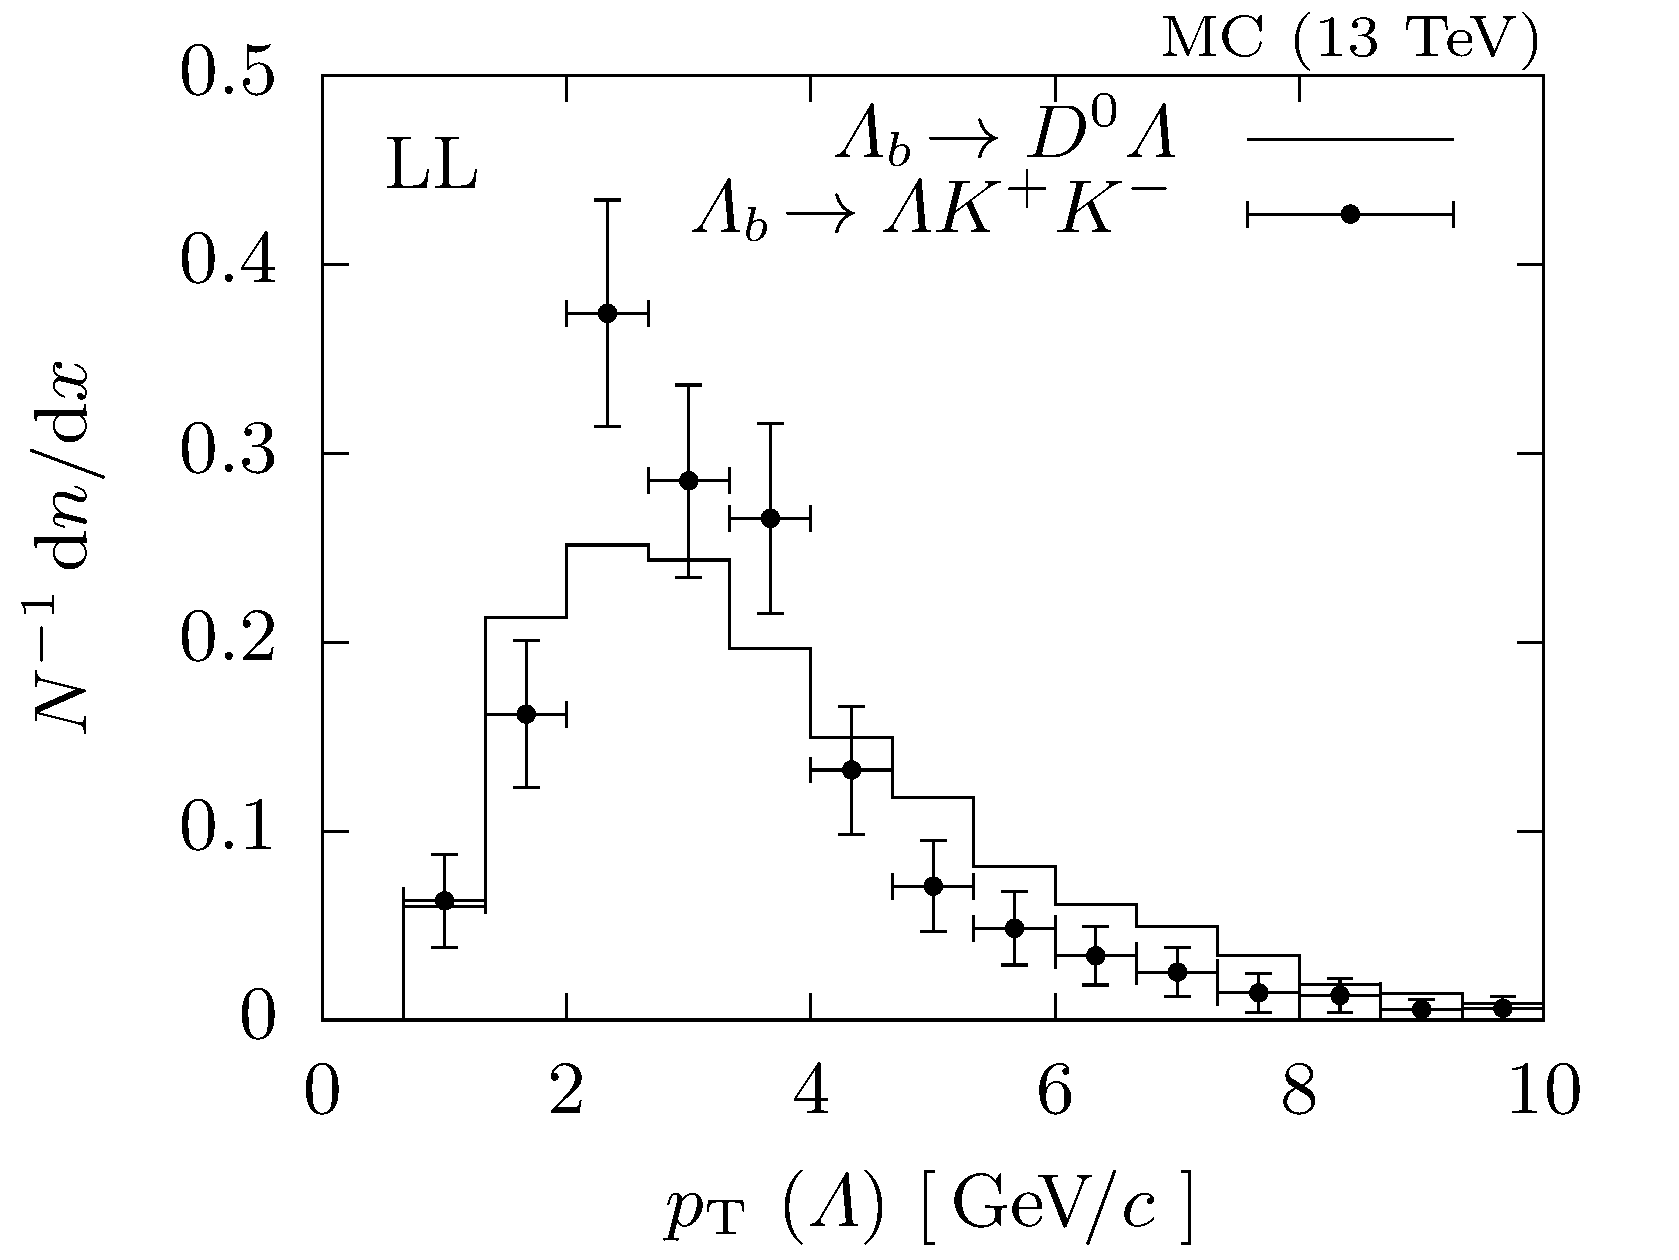
\includegraphics[scale=1.]{Lb2LzKK_bkg/hLzpT_LL.png}
    \end{subfigure}
    \begin{subfigure}{.49\textwidth}
        \centering
        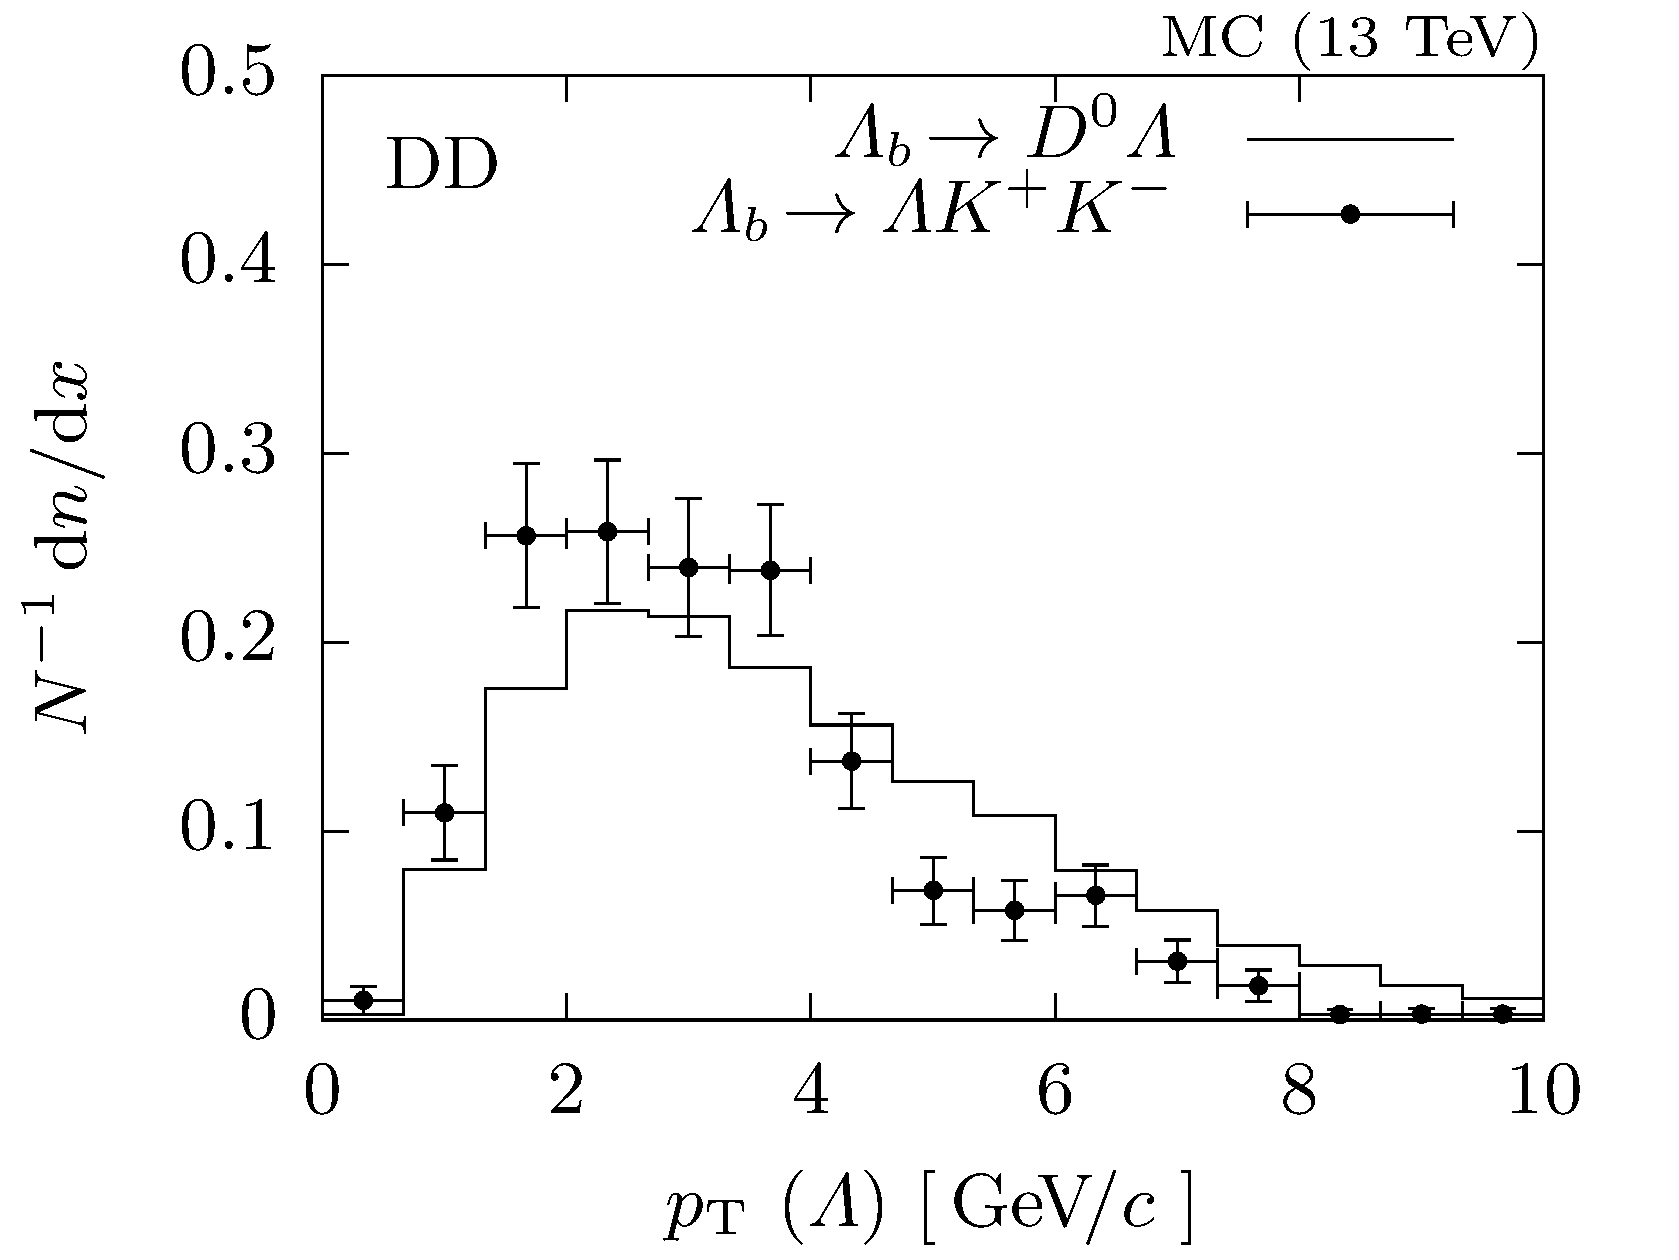
\includegraphics[scale=1.]{Lb2LzKK_bkg/hLzpT_DD.png}
    \end{subfigure}
    \caption{Transverse momentum distribution of \Lz baryons from \gls{mc} simulated \decay{\Lb}{\Dz\Lz} and \decay{\Lb}{\Lz\Km\Kp} decays. The distributions are normalized in order to compensate their largely different yields for the sake of comparison. The transverse momentum of the charmless three-body decay seemingly prefer smaller values (both for \gls{LL} tracks on the left, and \gls{DD} tracks on the right) for reasons we elaborate in Sec.~\ref{sec:apdx_charmlessrel_Lzp}.}
    \label{fig:apdx_charmlessrel_ptLz}
\end{figure}

\begin{figure}[htbp]
    \centering
    \begin{subfigure}{.49\textwidth}
        \centering
        %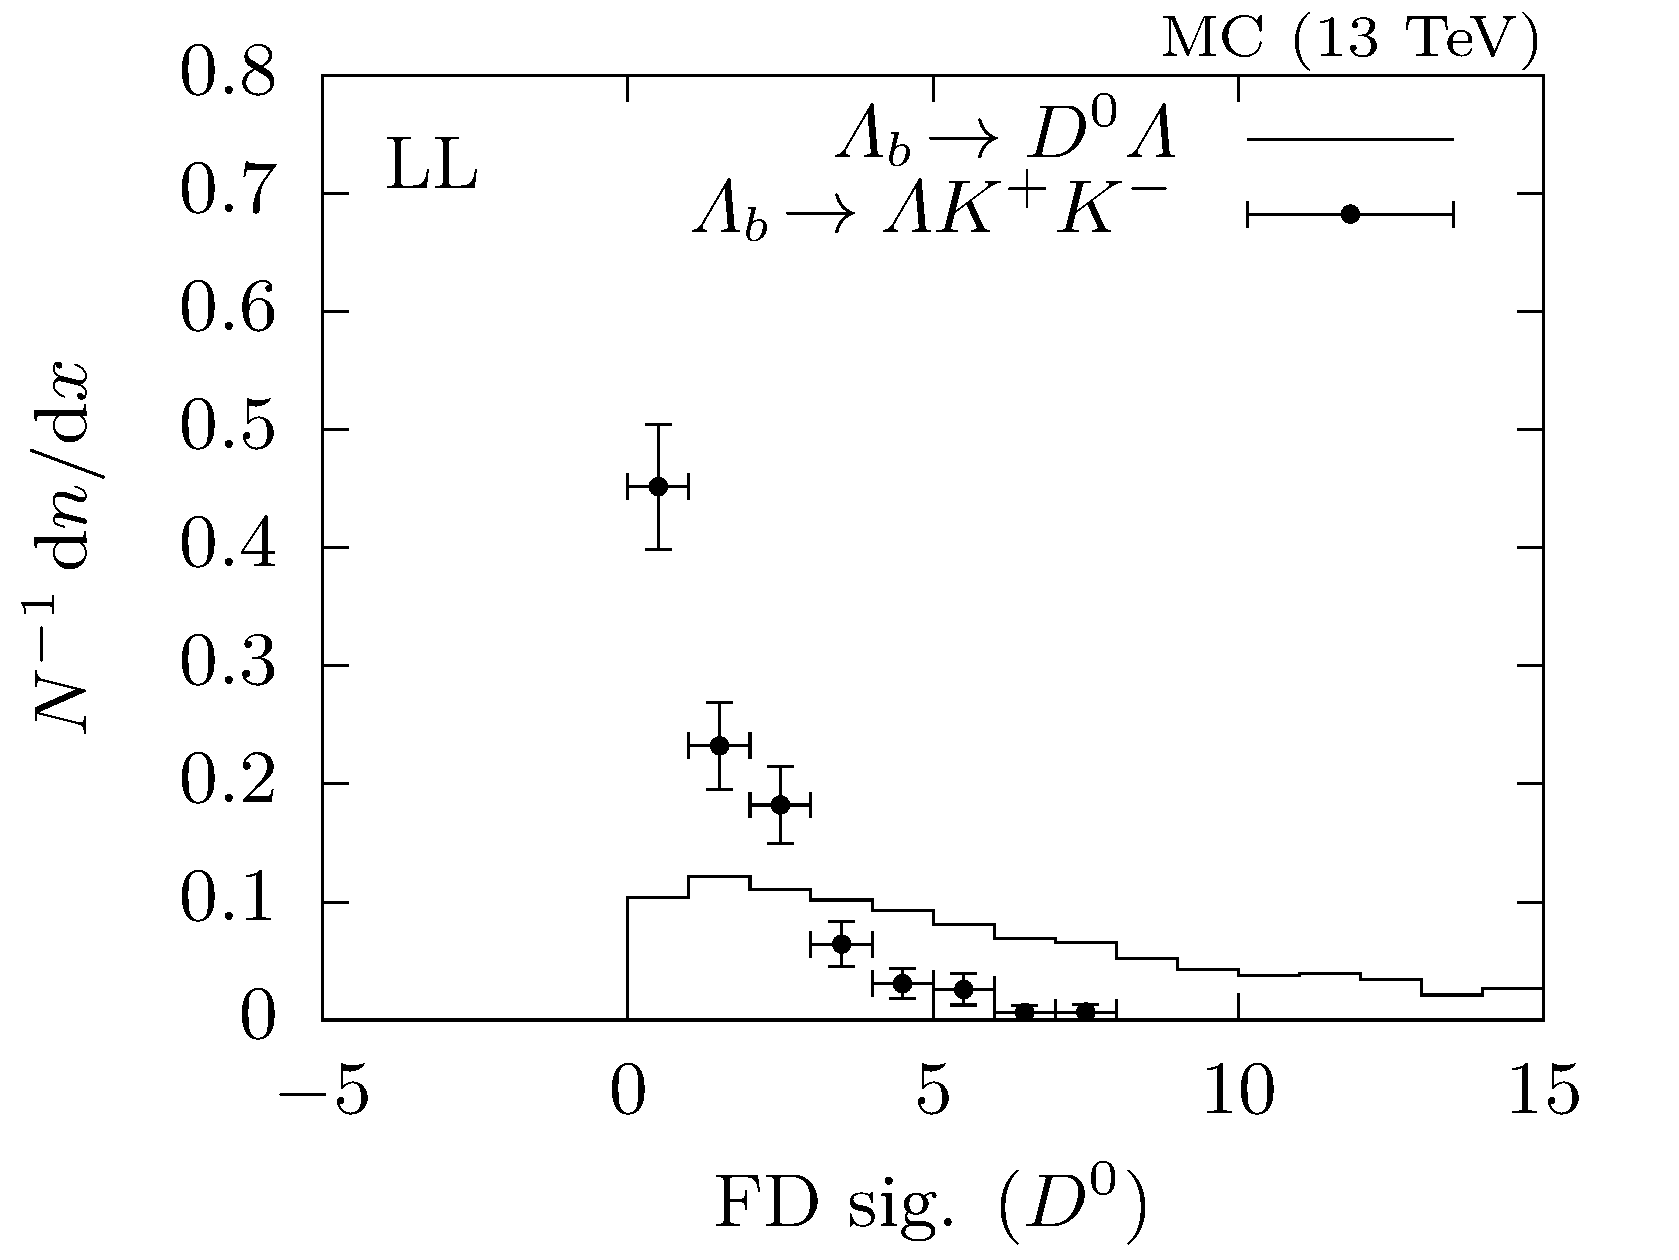
\includegraphics[scale=1.]{Lb2LzKK_bkg/hDzFDsig_LL.png}
        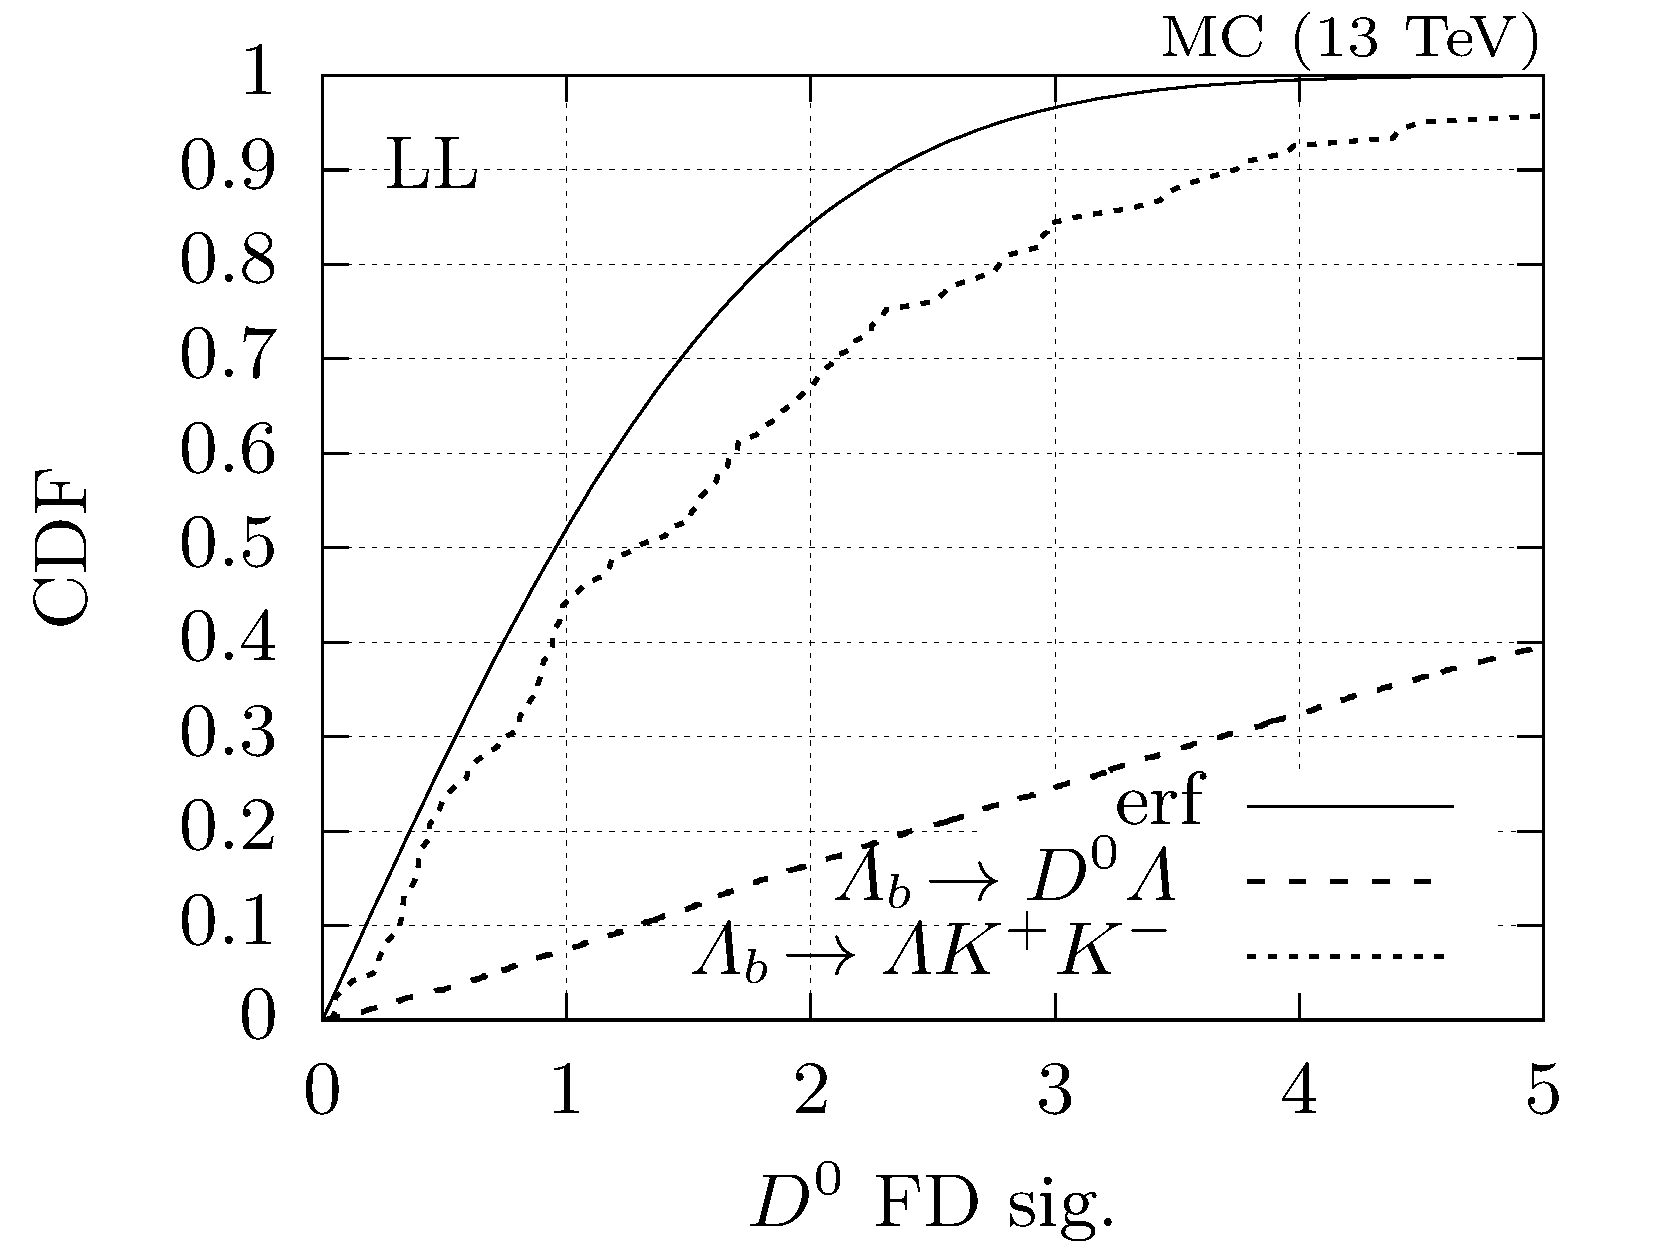
\includegraphics[scale=1.]{Lb2LzKK_bkg/hDzFDsig_cdf_LL_filtered.png}
    \end{subfigure}
    \begin{subfigure}{.49\textwidth}
        \centering
        %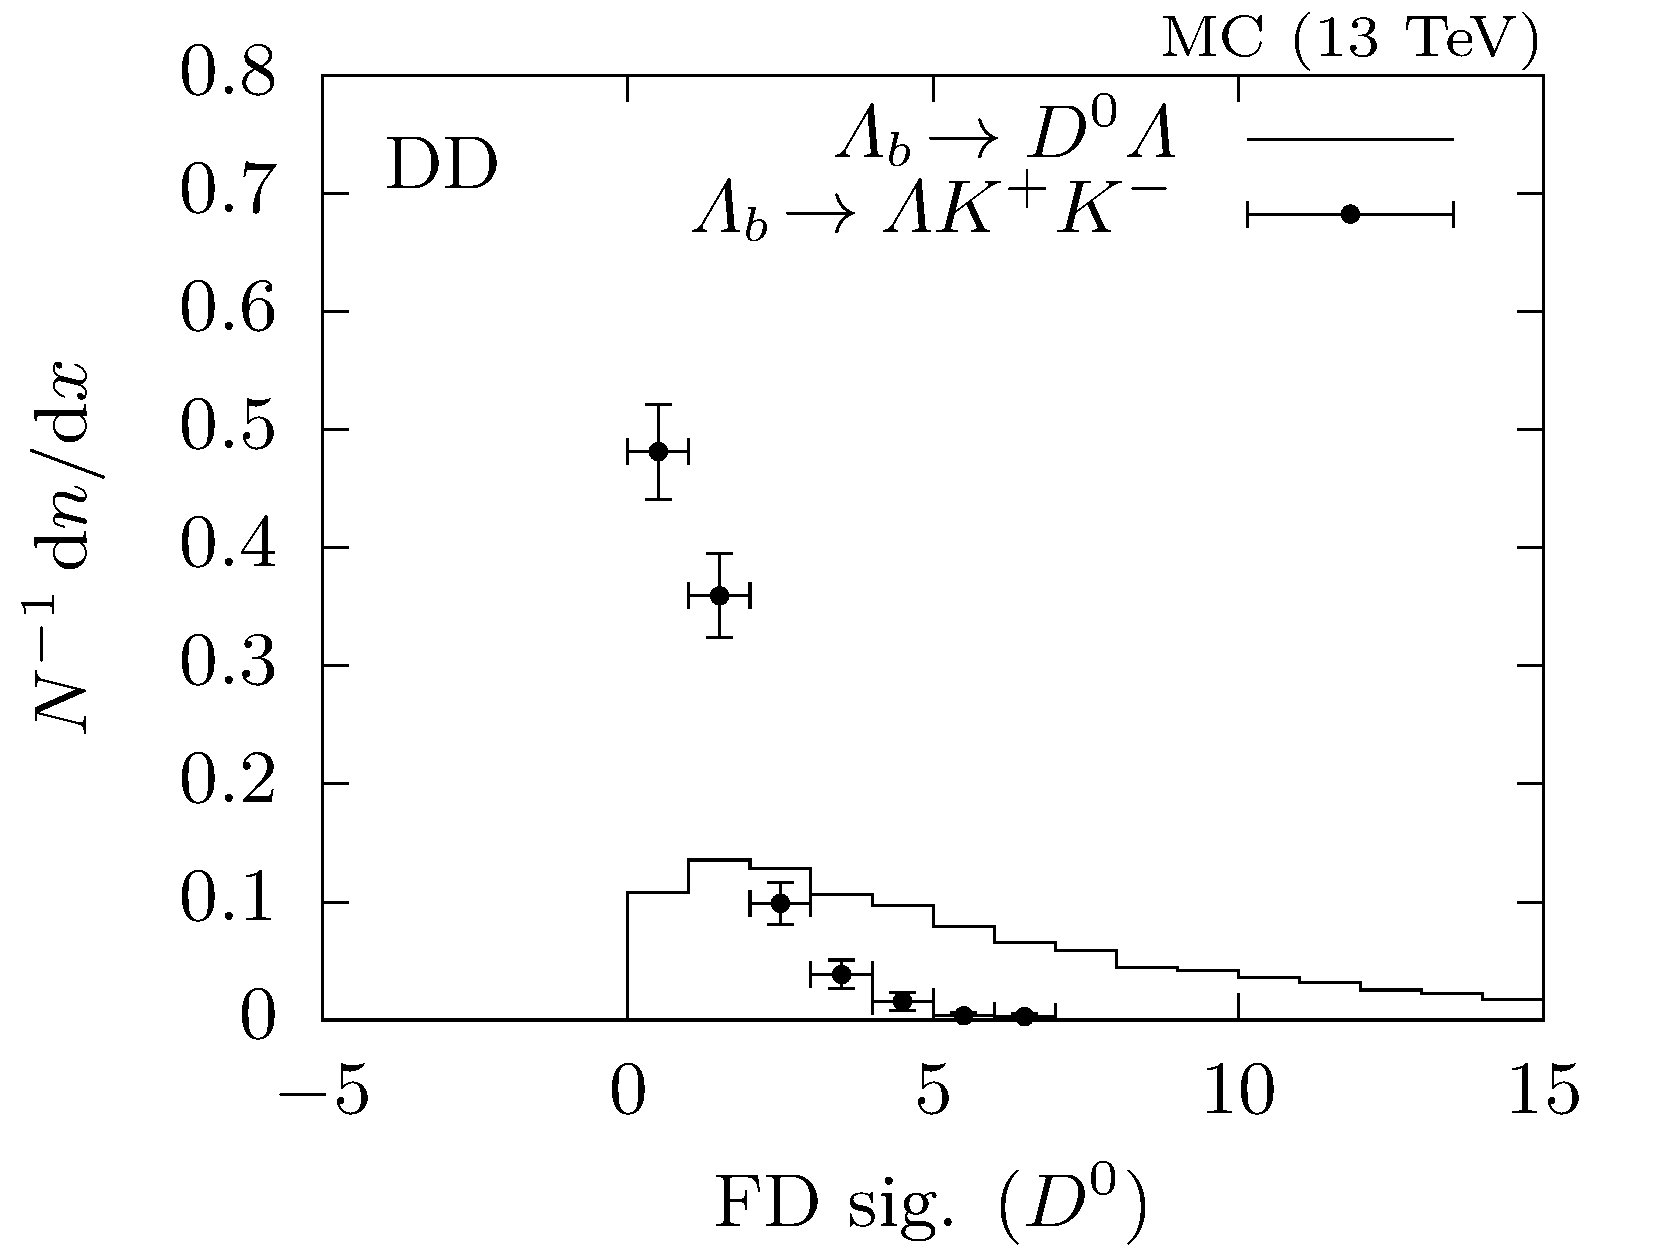
\includegraphics[scale=1.]{Lb2LzKK_bkg/hDzFDsig_DD.png}
        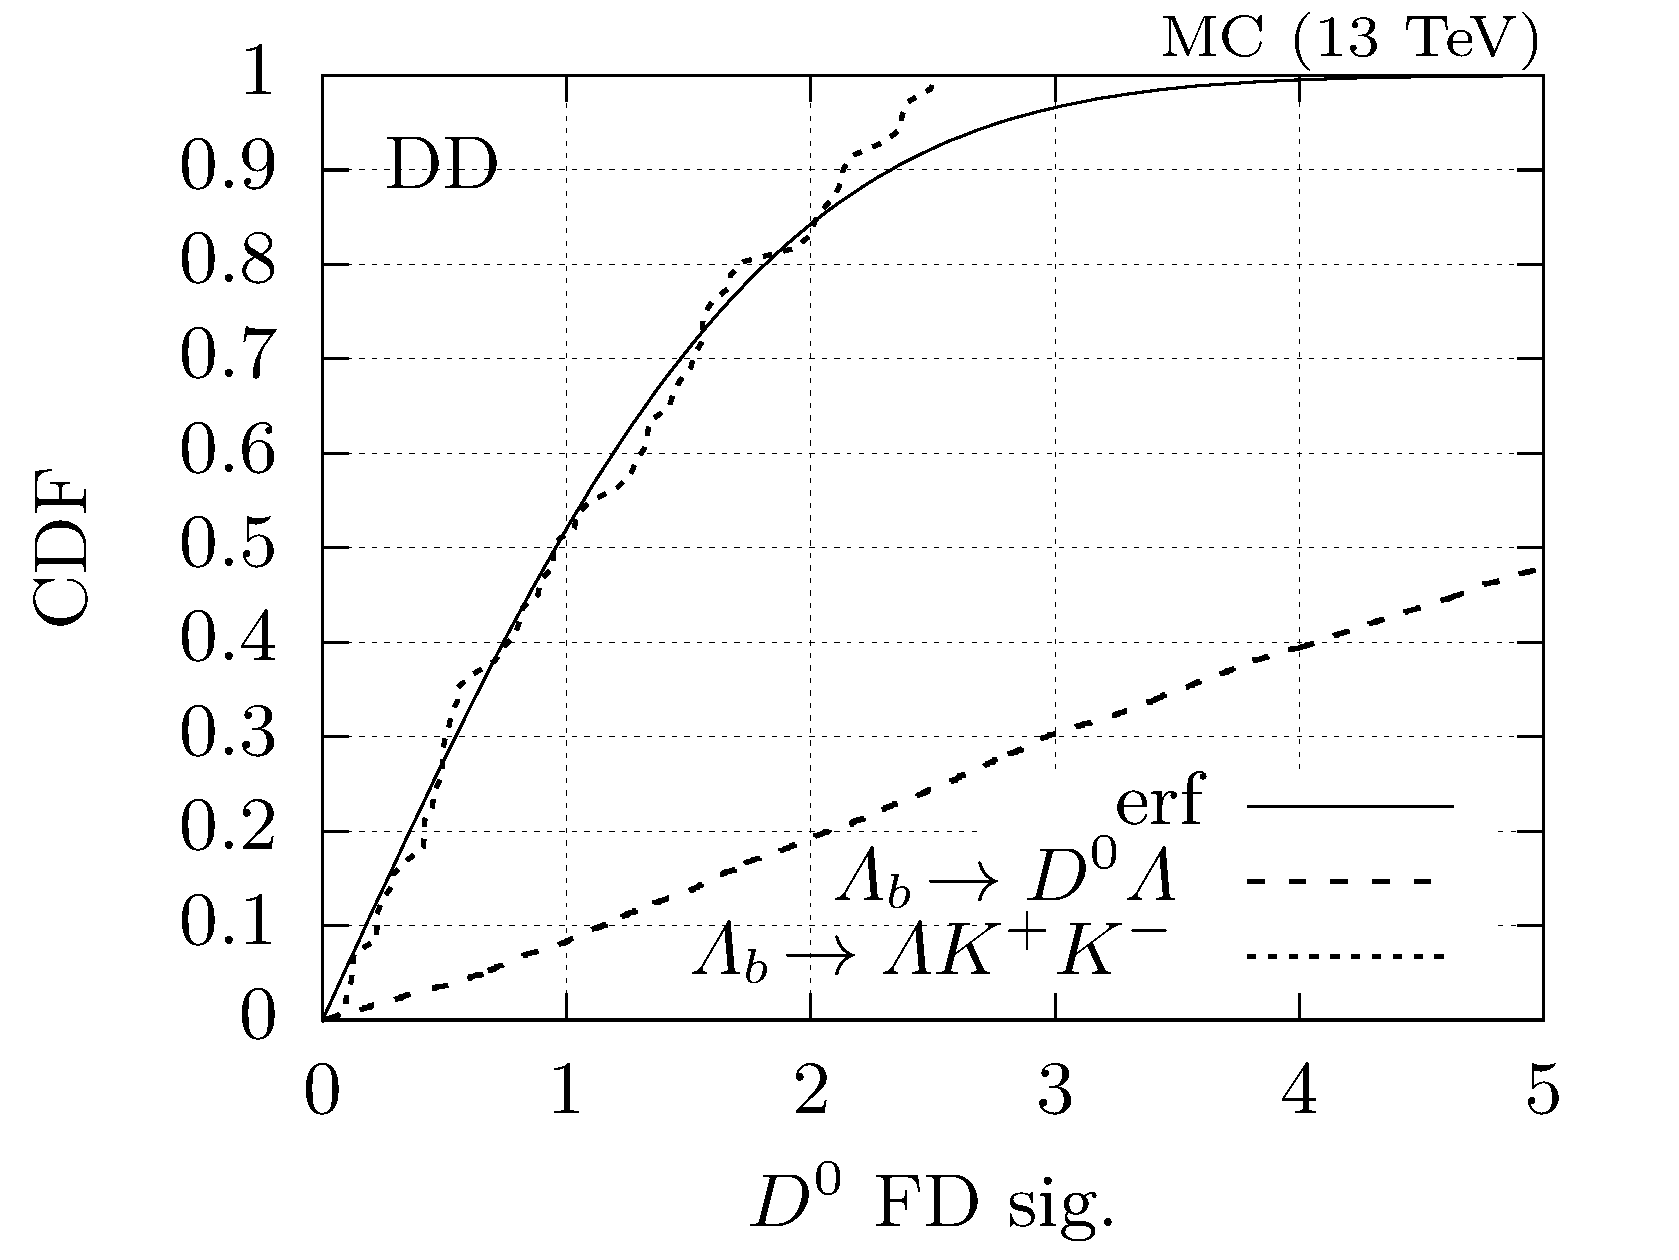
\includegraphics[scale=1.]{Lb2LzKK_bkg/hDzFDsig_cdf_DD_filtered.png}
    \end{subfigure}
    %\caption{Flight distance significance of \Dz mesons from MC simulated \decay{\Lb}{\Dz\Lz} and \decay{\Lb}{\Lz\Km\Kp} decays, where the latter is reflected as \decay{\Lb}{\Lz\Km\pip} and spuriously reconstructed as \decay{\Lb}{\Dz\Lz}. The distributions are normalized in order to compensate their largely different yields for the sake of comparison.}
    \caption{CDF of flight distance significance of \Dz mesons from \gls{mc} simulated \decay{\Lb}{\Dz\Lz} and \decay{\Lb}{\Lz\Km\Kp} decays where the latter is reflected as \decay{\Lb}{\Lz\Km\pip} and spuriously reconstructed as \decay{\Lb}{\Dz\Lz}. For comparison reason we also show the CDF of a Gaussian function (Error function).}
    \label{fig:apdx_charmlessrel_fdDz}
\end{figure}

In the present analysis, \decay{\Lb}{\Lz\Km\Kp} is considered a background, hence the implication of applying a \gls{dtf} assuming a decay tree \decay{\Lb}{\Dz\Lz} is of interest.
In the right part of Fig.~\ref{fig:apdx_charmlessrefl_pLz} we show the three-momentum magnitude of the \Lz baryon in the \Lb rest frame after applying such a \gls{dtf}.
Unsurprisingly, the values are smeared and shifted towards larger values.
As a consequence, the very same behavior is observed when comparing the invariant masses $m(\Dz\Lz)$ before and after applying the \gls{dtf}, shown in Fig.~\ref{fig:LbToLzKK_bkg_hLbM} and Fig.~\ref{fig:apdx_charmlessrel_mLb_dtf}, respectively.

\begin{figure}[htbp]
    \centering
    \begin{subfigure}{.49\textwidth}
        \centering
        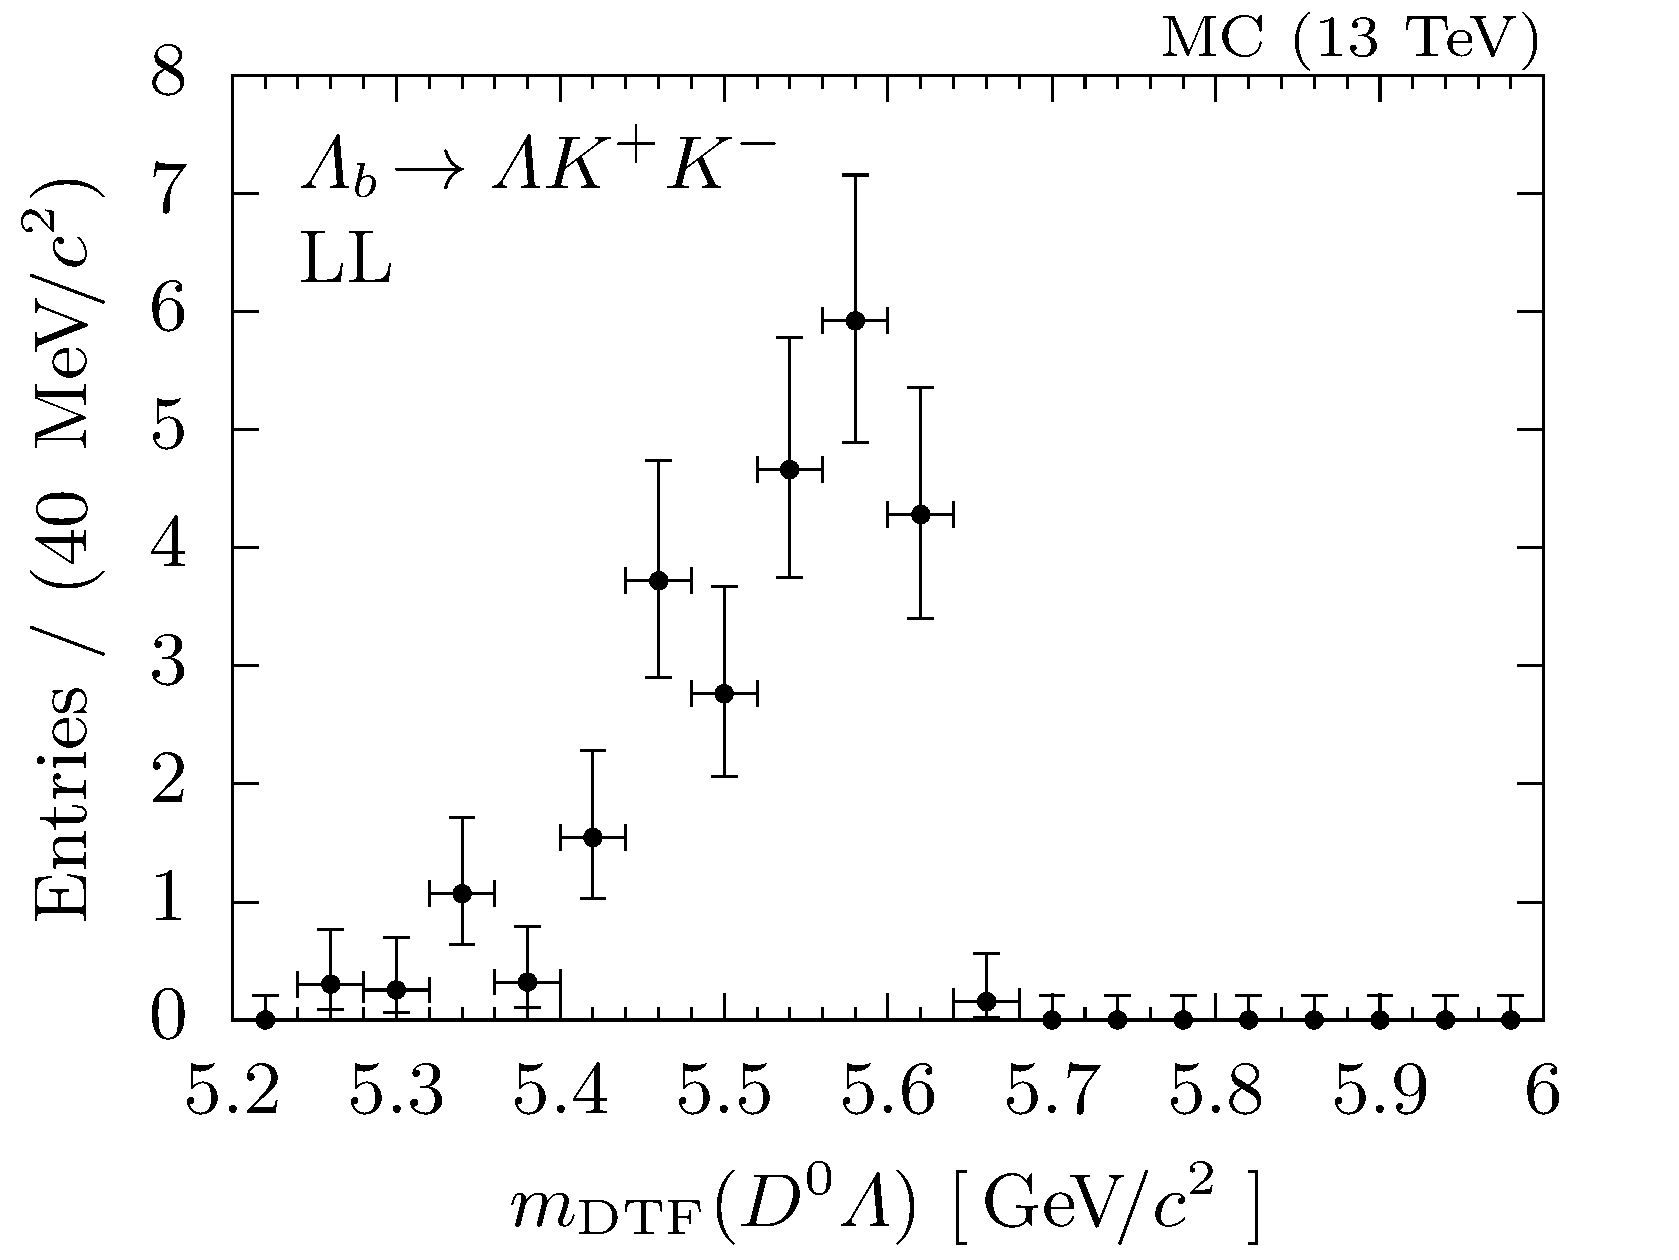
\includegraphics[scale=1.]{Lb2LzKK_bkg/hLb_dtf_M_LL.png}
    \end{subfigure}
    \begin{subfigure}{.49\textwidth}
        \centering
        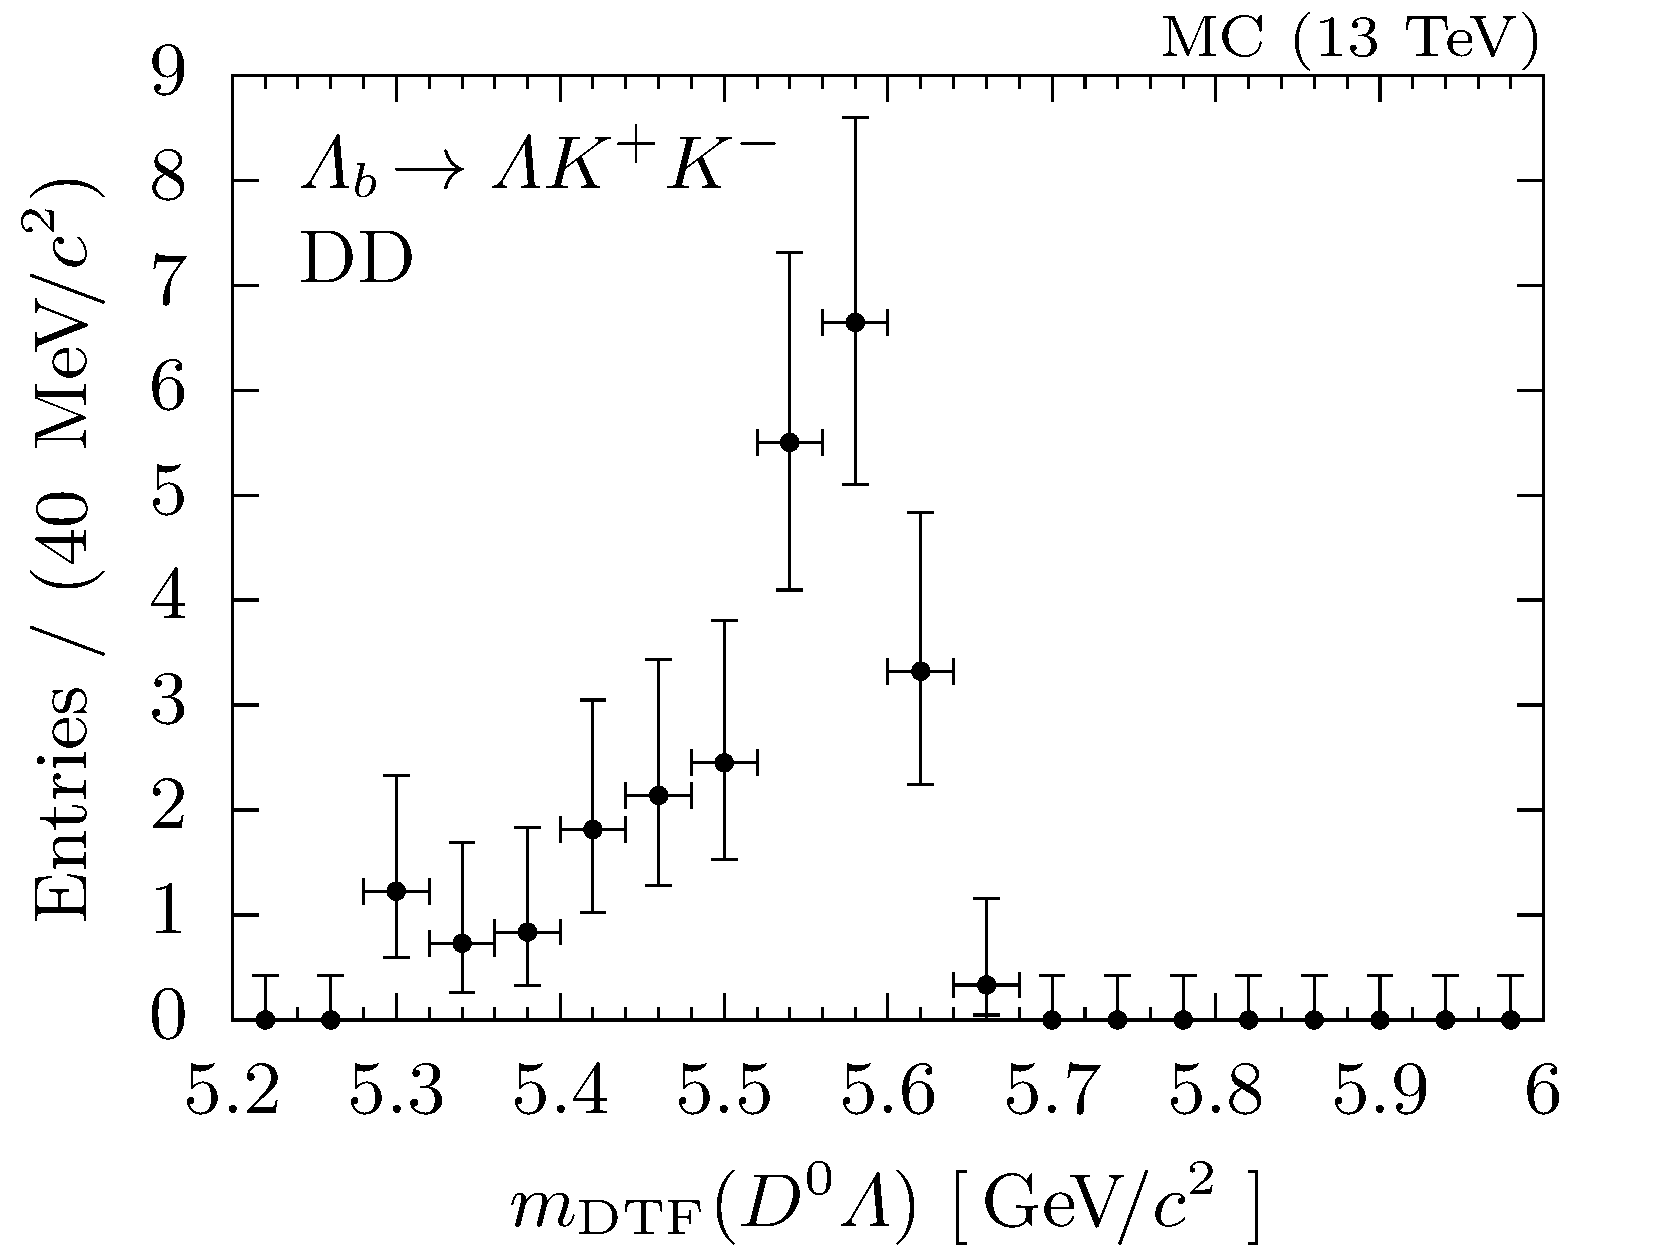
\includegraphics[scale=1.]{Lb2LzKK_bkg/hLb_dtf_M_DD.png}
    \end{subfigure}
    \caption{Combined invariant mass of \decay{\Dz}{\Km\pip} and \decay{\Lz}{\proton\pim} candidates from \gls{mc} simulated \decay{\Lb}{\Lz\Km\Kp} decays after applying a \gls{dtf} assuming the decay tree \decay{\Lb}{\Dz\Lz}.}
    \label{fig:apdx_charmlessrel_mLb_dtf}
\end{figure}

%\begin{figure}[htbp]
%    \centering
%    \begin{subfigure}{.49\textwidth}
%        \centering
%        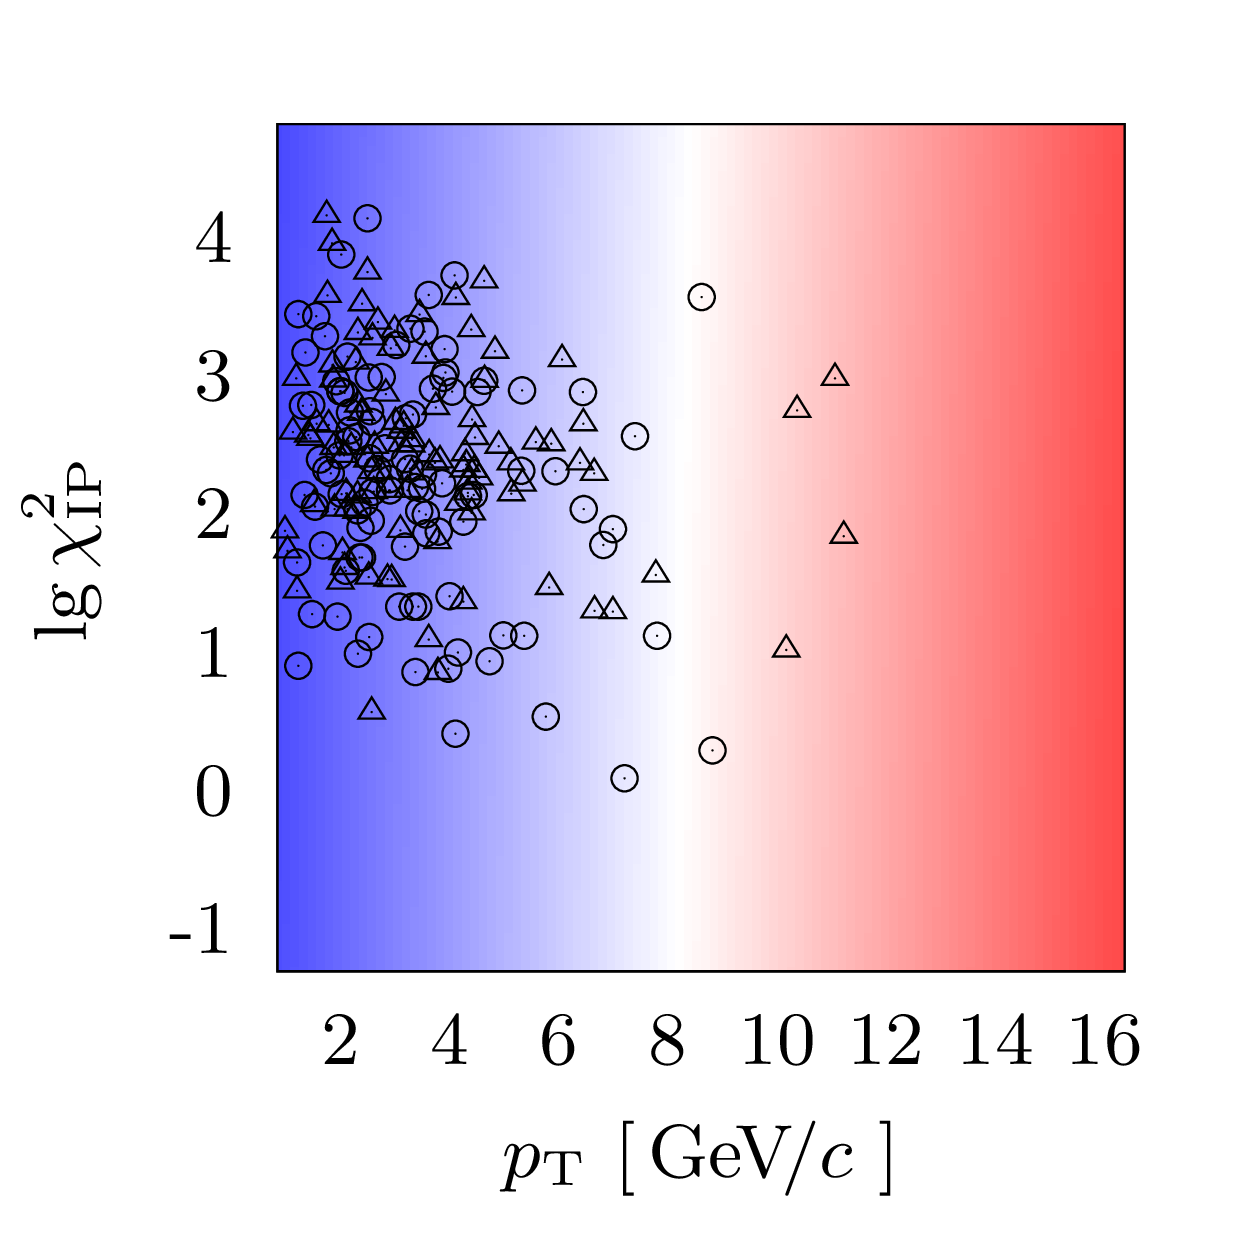
\includegraphics[scale=1.]{Lb2LzKK_bkg/top2features_clfLz_LL.png}
%    \end{subfigure}
%    \begin{subfigure}{.49\textwidth}
%        \centering
%        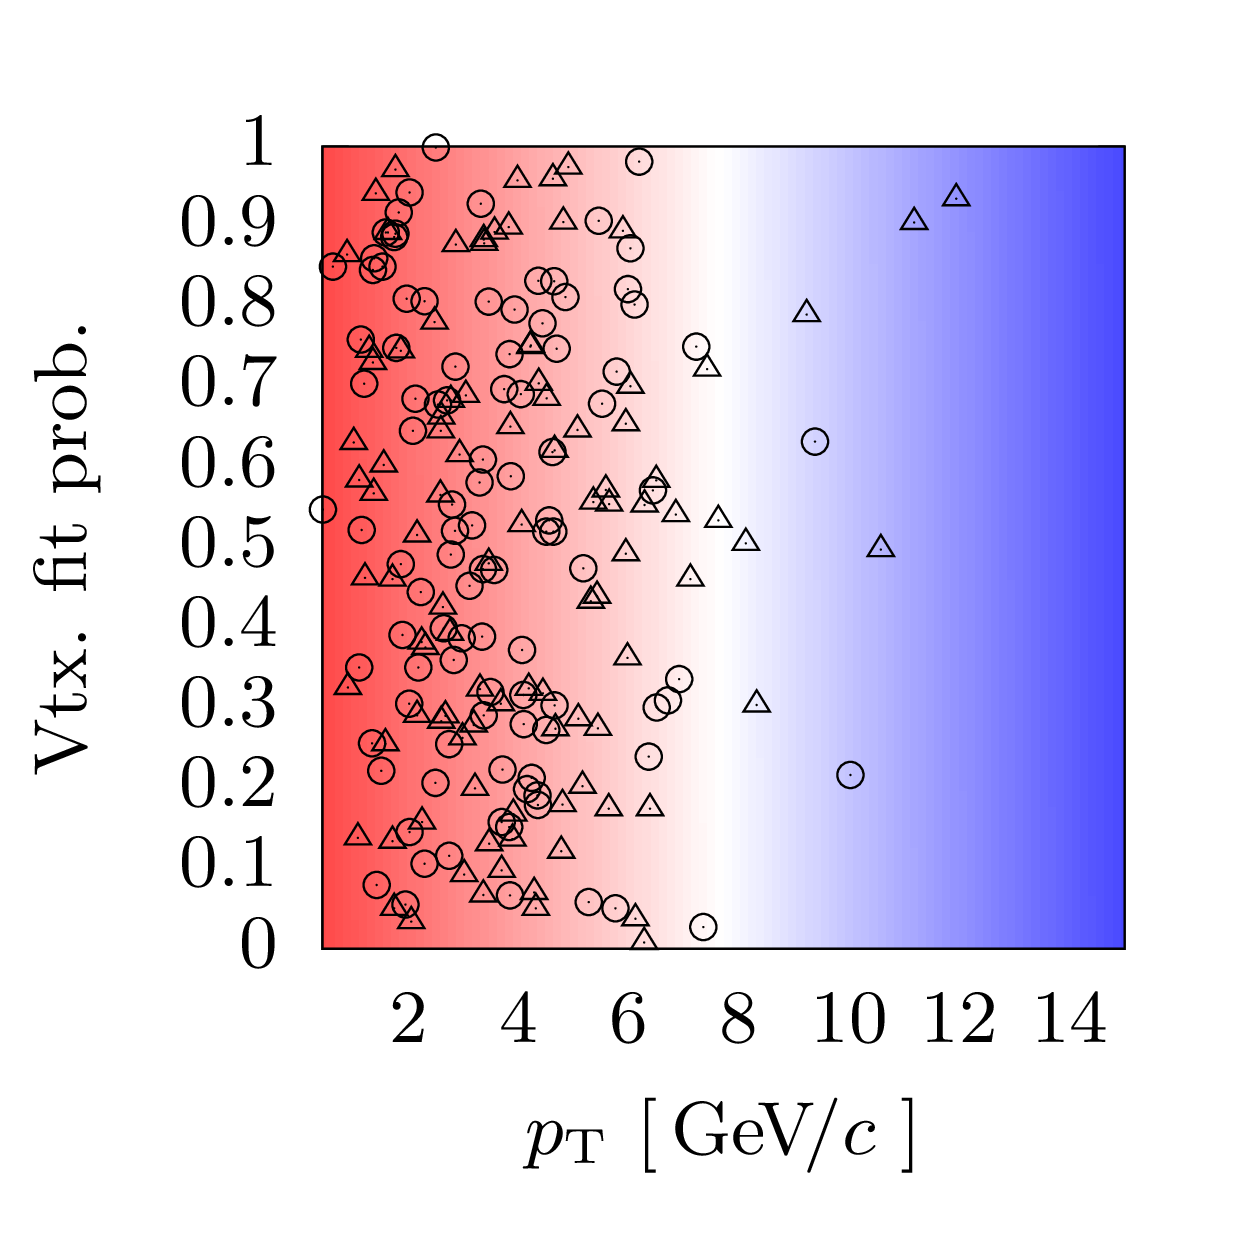
\includegraphics[scale=1.]{Lb2LzKK_bkg/top2features_clfLz_DD.png}
%    \end{subfigure}
%    \par\bigskip
%    \begin{subfigure}{.49\textwidth}
%        \centering
%        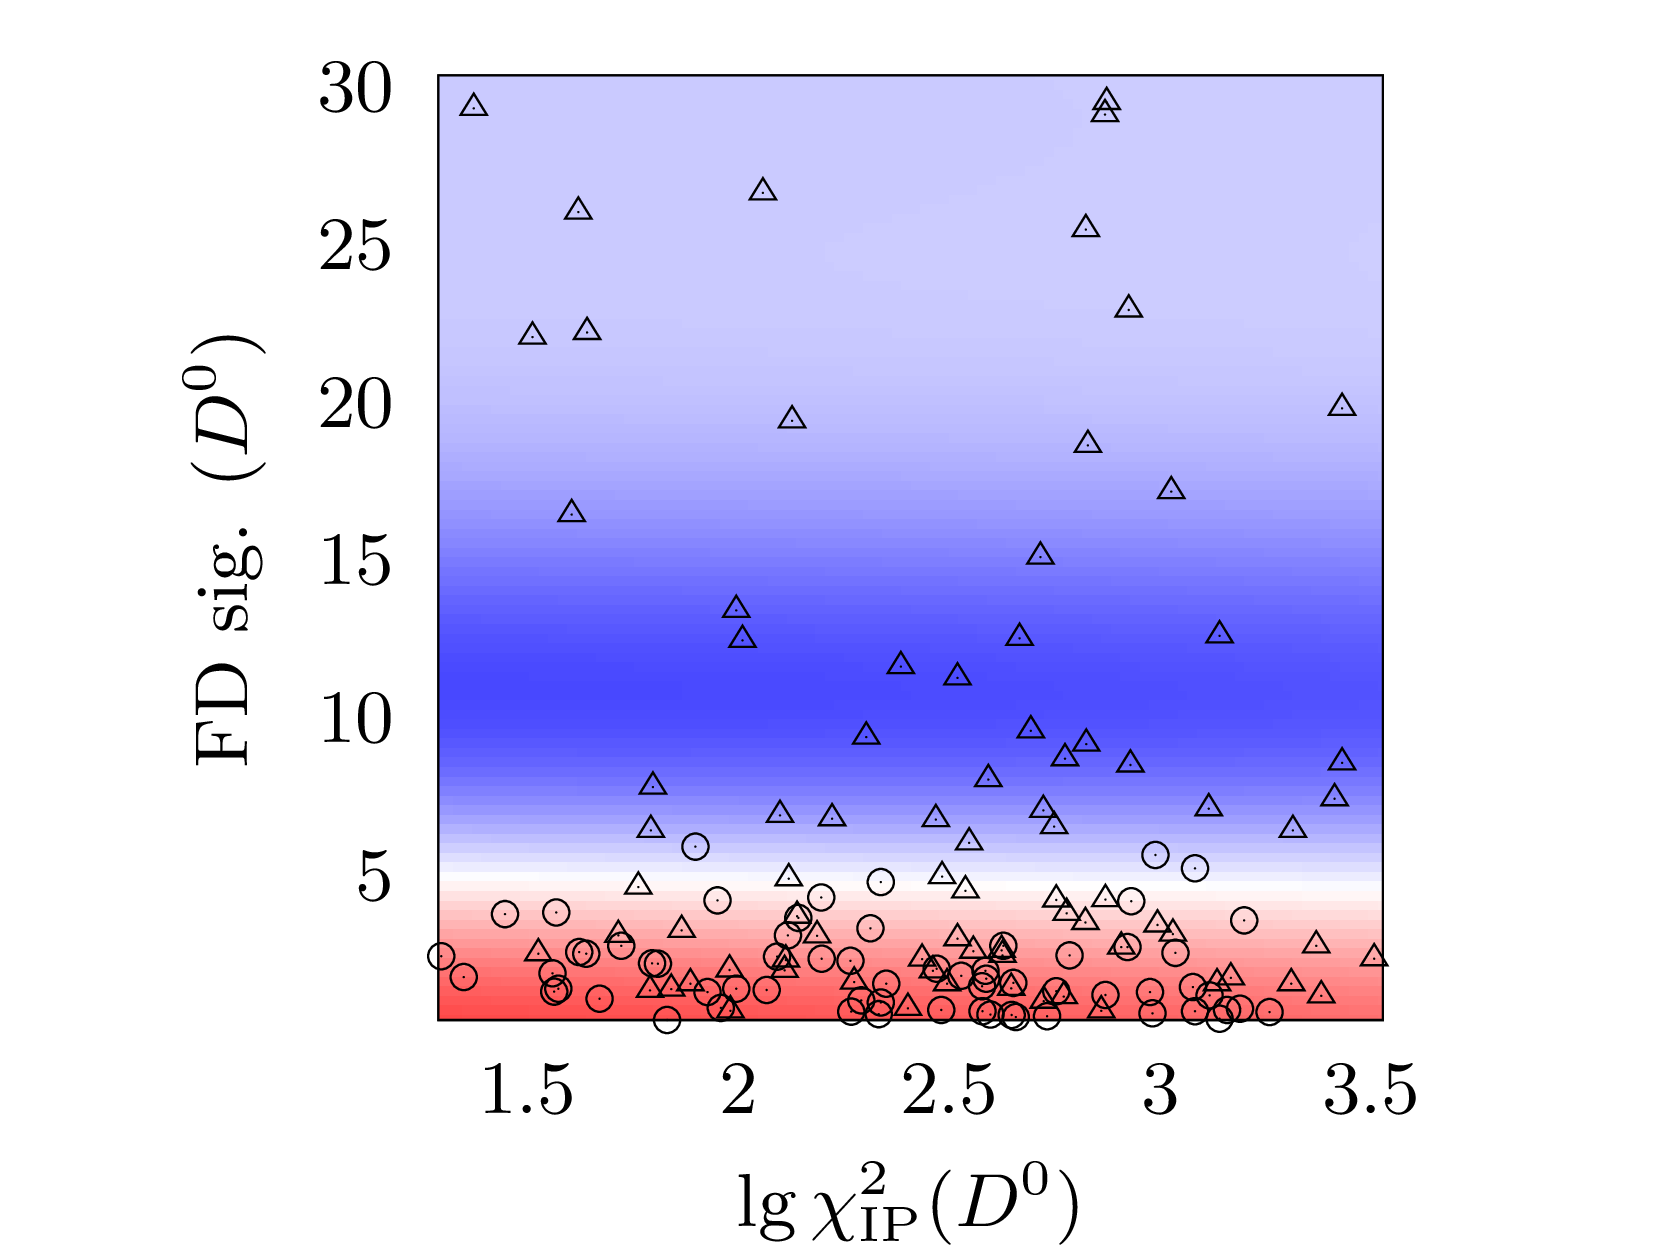
\includegraphics[scale=1.]{Lb2LzKK_bkg/top2features_clfLbDz_LL.png}
%    \end{subfigure}
%    \begin{subfigure}{.49\textwidth}
%        \centering
%        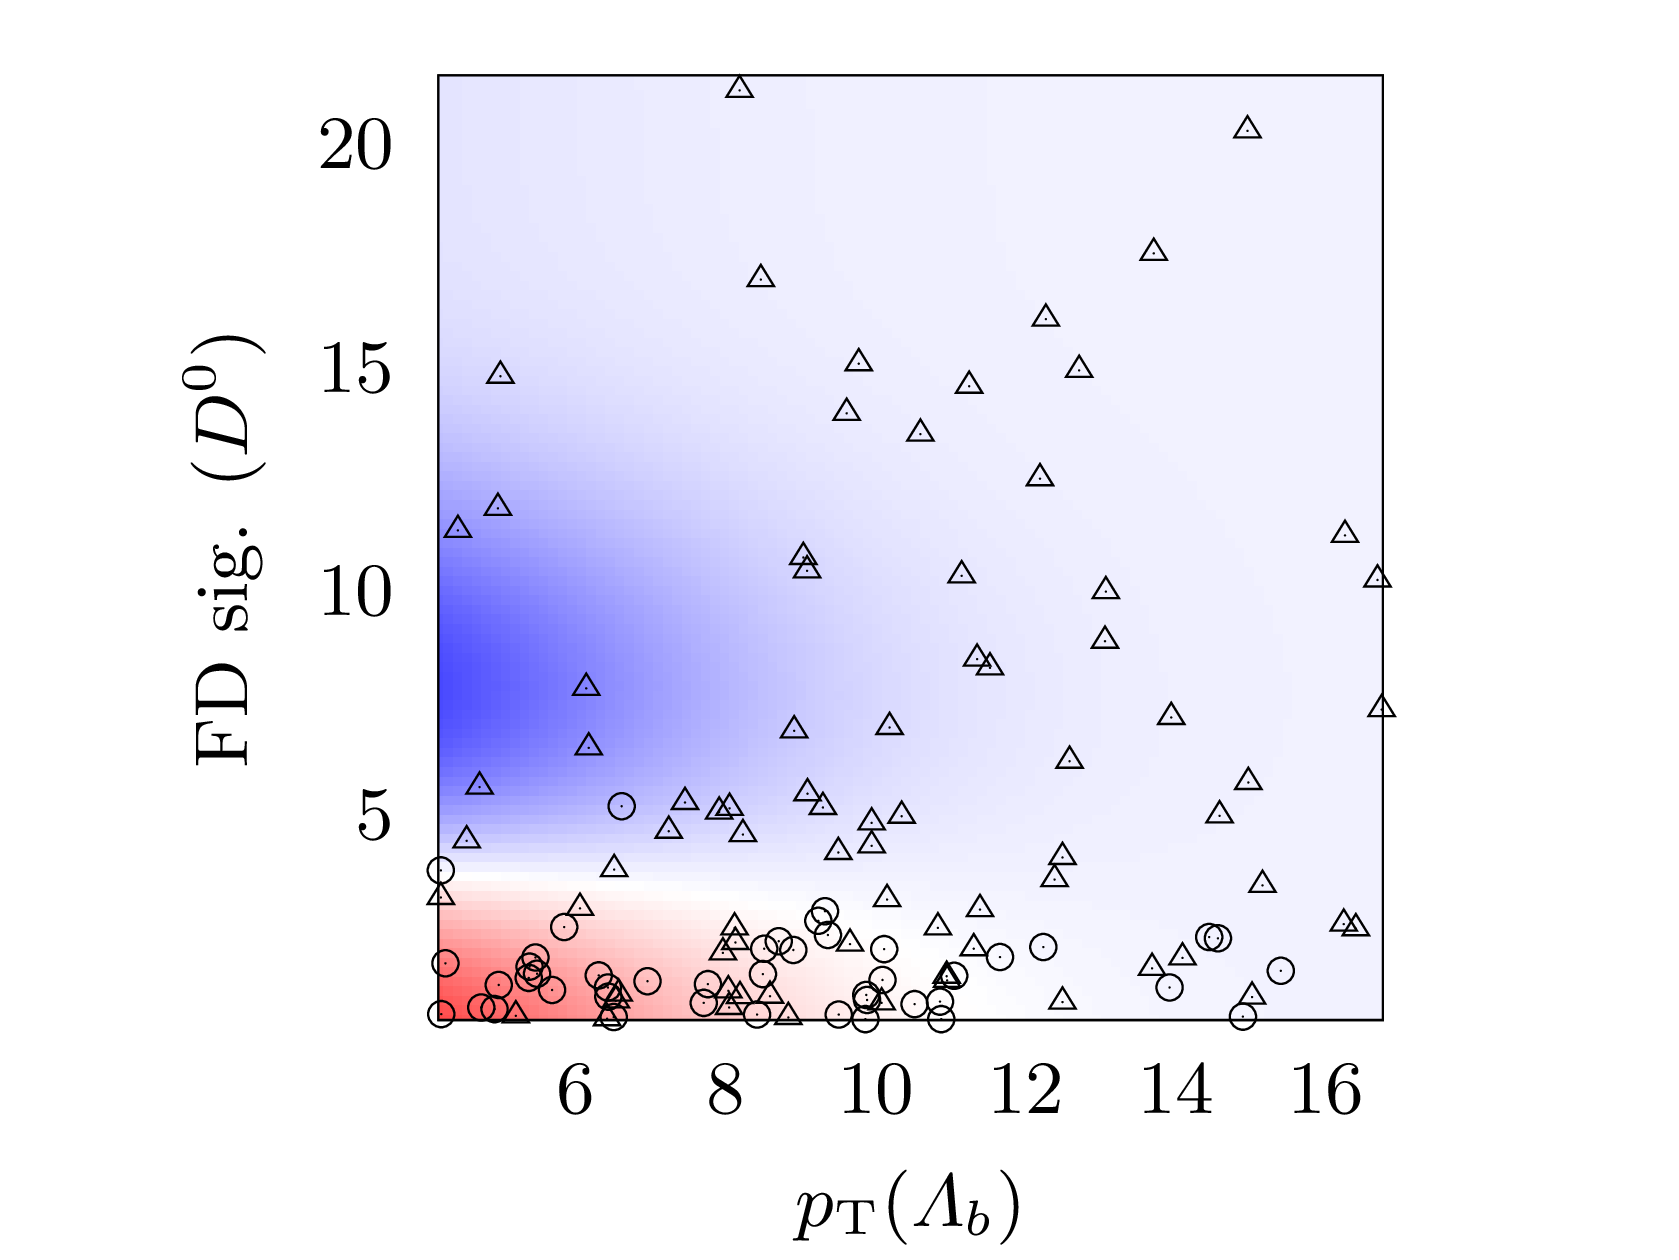
\includegraphics[scale=1.]{Lb2LzKK_bkg/top2features_clfLbDz_DD.png}
%    \end{subfigure}
%    \caption{}
%\end{figure}
